\documentclass[USenglish]{article}

%\usepackage[utf8]{inputenc}
\RequirePackage[no-math]{fontspec}

\usepackage[small]{dgruyter}
\usepackage{microtype}
\usepackage{enumerate}
\usepackage{eqnarray}

\newcommand{\wrt}{w.\,r.\,t.\ }
\newcommand{\Wrt}{W.\,r.\,t.\ }
\newcommand{\eg}{e.\,g.,}
\newcommand{\Eg}{E.\,g.,}
\newcommand{\ie}{i.\,e.,}
\newcommand{\Ie}{I.\,e.,}
\newcommand{\Sub}[1]{\ensuremath{\mathrm{_{#1}}}}
\newcommand{\Sup}[1]{\ensuremath{\mathrm{^{#1}}}}
\newcommand{\Subsf}[1]{\ensuremath{\mathsf{_{#1}}}}
\newcommand{\Supsf}[1]{\ensuremath{\mathsf{^{#1}}}}
\newcommand{\pPB}{p\Subsf{PB}}

\newcommand{\NACb}{NAC\Sub{bare}}
\newcommand{\NACa}{NAC\Sub{adj}}
\newcommand{\PGCd}{PGC\Sub{det}}
\newcommand{\PGCa}{PGC\Sub{adj}}

\newcommand*\Rot{\rotatebox{75}}

\usepackage{gb4e-}

\usepackage{bbding}
\newcommand{\CheckIt}{\CheckmarkBold}


\usepackage{natbib}
\bibliographystyle{./unified}

\begin{document}

  %\articletype{...}

  \author*[1]{Roland Schäfer}
  %\runningauthor{...}
  \affil[1]{Freie Universität Berlin}
  \title{Competing Constructions for German Measure Phrases}
  \runningtitle{Competing Constructions for German Measure Phrases}
  %\subtitle{...}
  \abstract{In German, nominal morpho-syntax\ldots}
  \keywords{alternations, hierarchical models, corpus methods and experimental methods, measure constructions, German}
  %\classification[PACS]{...}
  %\communicated{...}
  %\dedication{...}
  %\received{...}
  %\accepted{...}
  \journalname{(submitted)}
  \journalyear{2017}
  %\journalvolume{...}
  %\journalissue{...}
  %\startpage{...}
  %\aop
  %\DOI{...}


  
\maketitle



%%%%%%%%%%%%%%%%%%%%%%%%%%%%%%%%%%%%%%%%%%%%%%%%%%%%%%%%%%%%%%%%%%%%%%%
%%%%%%%%%%%%%%%%%%%%%%%%%%%%%%%%%%%%%%%%%%%%%%%%%%%%%%%%%%%%%%%%%%%%%%%
%%%%%%%%%%%%%%%%%%%%%%%%%%%%%%%%%%%%%%%%%%%%%%%%%%%%%%%%%%%%%%%%%%%%%%%


\section{Cognitively oriented corpus linguistics: theories, case studies, and methods}
\label{sec:cogocl}

\subsection{Corpora and cognition}

This paper deals with a morpho-syntactic alternation that occurs only in a very specific syntactic measure noun phrase construction.
By \textit{alternation} I refer to a situation where two or more forms or constructions are available with no clear difference in acceptability, function, or meaning.
I use it as an example case for a protocol for the estimation and validation of corpus-based models in cognitively oriented corpus linguistics.
I briefly motivate this approach in this introduction, for details see Section~\ref{sec:cocl}.

In German grammar, the term \textit{Zweifelsfälle} `cases of doubt' is often used \citep{Klein2009}.

% Add to CogL special issue: Look at what non-cognitivists do
% => their have interesting data and interesting generalisations (which are not intrinsically nonsense or incompatible with CogLi)
% => where they lack is modelling probabilistic effects, and that should be one of the strengths of cognitively oriented (corpus) linguistics
% => FUZZINESS and SIMILARITY in classification (prototypes and exemplars)
% => advantage: testable with corpus and experiment (ideally both)

% This is a case study and more.
% => gathering a descriptive picture from non-cognitive literature
% => motivating the phenomenon as relevant for CogLi
% => careful protocol for:
%  =>> motivating range of alternants under examination and selecting hypotheses (sound and/or slightly less sound, but MAKE CLEAR what they are!)
%  =>> motivate whether larger utterance context plays a role or not (sociolinguistic & register(?) commitment)
%  =>> choosing right data
%  =>> choosing "the right" – NO, "some appropriate" statistics
%  =>> getting minimal external validation with experiments

% This article attempts to follow this protocol as well as possible given the available analyses/data sources/nature of the phenomenon.

%%%%%% From old structure:
%
%\subsection{Cognitively oriented corpus linguistics}
%\label{sec:cocl}
%
% Mention: Corpus-as-input is OK as a hypothesis but NOT as a research programme
% Entrenchment_Stefanowitsch and Flach for submission + Schmid C2C
%  => otherwise any spurious pattern found in corpora (meeting certain criteria)
%  => is automatically "cognitive"
%
%Following the descriptive introduction to the measure noun phrase alternation in Section~\ref{sec:germanmeasurenps}, this section situates the work presented here within the broader theoretical context of what can be called \textit{cognitively oriented corpus linguistics}.
%
%Unless there are strong, numeric, and cognitively motivated hypotheses, some experimental validation is required to make a corpus study \textit{cognitive} in any sense.
%Assuming the \textit{corpus as input} hypothesis without experimental validation is completely unsound in as much as researcher could extract any arbitrary -- often spurious -- usage pattern from a (usually noisy) corpus and claim that it has a cognitive reality.
%
% Cite:
% [Cognitive Linguistics] Similarity in linguistic categorization- The importance of necessary properties
% 10.1.1.980.9935
% __IMP__Measurenouns__cog-2015-0101
%
% Maybe:
% [Cognitive Linguistics] The processing of verb-argument constructions is sensitive to form, function, frequency, contingency and prototypicality
% [Cognitive Linguistics] Alternation-based generalizations are stored in the mental grammar- Evidence from a sorting task experiment //// along with CApelle's allostructions
%
% Method:
% Noble


%%%%%%%%%%%%%%%%%%%%%%%%%%%%%%%%%%%%%%%%%%%%%%%%%%%%%%%%%%%%%%%%%%%%%%%
%%%%%%%%%%%%%%%%%%%%%%%%%%%%%%%%%%%%%%%%%%%%%%%%%%%%%%%%%%%%%%%%%%%%%%%

\subsection{A word on statistical analysis}
\label{sec:rightstatistics}

In this section, I briefly motivate the choice of statistical models which I use later in Section~\ref{sec:corpusstudies}.
In the spirit of the careful and methodologically sound approach to cognitively oriented corpus linguistics laid out in Section~\ref{sec:cogocl}, authors should always provide at least a minimal motivation as part of the standard protocol, especially if there are alternative methods.

% NO to exploratory methods if we have hypotheses
% Testing (hypotheses about signs of regressors)
% Estimation => bootstrapping
% Model selection
%  => random vs fixed is not so simple, rather matter of getting model to converge
%  => Maximality
%  => NO to Gries 2015
% Model evaluation
% VS: Bayesian hype (Levshina)
% VS: alternative math (R-W)

% Cite:
% __IMP__Measurenouns__cog-2015-0054 (Levshina)
% [Cognitive Linguistics] Towards cognitively plausible data science in language research (NDL)

% Stats:
% BarrEa_RandomEffectsStructure_2014_JMemLang
% ContentServer (1)
% importatn_quotes
% Menard_2000-Coefficients_of_Determination_for_Multiple_Logistic_Regression_Analysis

%In the following, I examine the case alternation in German measure NPs under a cognitively oriented corpus linguistic perspective.
%Since, however, the statistical tool kit (hierarchical generalised linear models, general tools such as $p$ values and confidence intervals, resampling techniques, model selection and model evaluation strategies, alternative algorithms for estimation, etc.) is heterogeneous and often criticised (especially under noisy conditions and when researcher run the risk of doing data mining instead of proper theory testing) I present a careful protocol for specifying, estimating, validating, and interpreting such models in Section \ref{sec:corpusstudies}.

Before discussing the results in Section~\ref{sec:corpusstudies}, I show how I made sure that the relevant data is contained in the sample in Section \ref{sec:gettingdata}.

%\subsection{Tools for modelling alternations}
%\label{sec:righttools}
%
%In this section, I discuss the relevant statistical approaches to modelling alternations based on corpus data.
%I mainly focus on well-established Generalised Linear Models (GLMs) and their \textit{multi-level} or \textit{hierarchical} extensions, which are also called \textit{mixed models} (GLMMs).
%
%% TODO CONTENT HERE
%
%In Section~\ref{sec:corpusnonhierarchicalmodel}, I briefly discuss why a non-hierarchical model -- while it is an option in principle -- has serious disadvantages for the data set under discussion (and similar data sets).
%In Section~\ref{sec:corpushierarchicalmodel}, I present the hierarchical model which is actually interpreted as the primary result of this study.
%Section~\ref{sec:bayesian} takes a short detour and shows (by example) that results from Bayesian estimation are not intrinsically different from those obtained from Maximum Likelihood methods, although Bayesian approaches have recently been touted to solve various problems facing applied statistics in various fields, even including cognitively oriented corpus linguistics.
%Finally, I summarise and interpret the results of the corpus study in Section~\ref{sec:interpretation}.






%%%%%%%%%%%%%%%%%%%%%%%%%%%%%%%%%%%%%%%%%%%%%%%%%%%%%%%%%%%%%%%%%%%%%%%
%%%%%%%%%%%%%%%%%%%%%%%%%%%%%%%%%%%%%%%%%%%%%%%%%%%%%%%%%%%%%%%%%%%%%%%
%%%%%%%%%%%%%%%%%%%%%%%%%%%%%%%%%%%%%%%%%%%%%%%%%%%%%%%%%%%%%%%%%%%%%%%


\section{Case assignment in German measure NPs}
\label{sec:germanmeasurenps}


\subsection{Two stable cases and a case alternation}
\label{sec:descriptive}

The alternation phenomenon to be discussed in this paper appears to be a straightforward case alternation at first sight.
However, without a solid knowledge of German nominal morpho-syntax, some of the more subtle distinctions that have to be made in its analysis can be confusing.
Therefore, I introduce and illustrate the relevant constructions in some detail in this section.
I describe the narrow range of syntactic constellations in which the alternation occurs, and I motivate the focus on \textit{only} this narrow (range rather than, for example, the whole range of nominal constructions expressing quantities).

I use the term \textit{measure noun phrase} (MNP) to refer a noun phrase (NP) in which a kind-denoting (count or mass) noun depends on another noun specifying a quantity of the objects or the substance denoted by the kind noun.
I call the kind-denoting noun simply the \textit{kind noun} and the quantity-denoting noun the \textit{measure noun}.
Measure nouns can be all sorts of nouns which genuinely denote a quantity (such as \textit{litre} or \textit{amount}) but also nouns denoting containers, collections, etc. (such as \textit{glass} or \textit{bucket}).
In a similar vein, \citet[284]{Brems2003} considers nouns as measure nouns \textit{which, strictly speaking, do not designate a `measure', but display a more nebulous} (\textit{sic!}) \textit{potential for quantification} (see also \citealp[530]{Koptjevskaja2001}, and \citealp[338]{Rutkowski2007}).
For illustration purposes, in the English \textit{a cup of fine coffee}, \textit{cup} is the measure noun, and \textit{coffee} is the kind noun.

In the case at hand, three different syntactic configurations need to be distinguished \wrt case assignment inside German measure noun phrases.
If the kind noun forms an NP with a determiner, the construction resembles (and is usually called) a \textit{pseudo-partitive} (on partitives and pseudo-partitives see, e.\,g., \citealp{Barker1998,Selkirk1977,Stickney2007,Vos1999}; for a recent application of the terminology to German, see \citealp{Gerstenberger2015}).%
\footnote{If the kind noun is definite, the construction instantiates a true partitive.
Whereas partitives are constructions denoting a proper part-of relation strictly requiring a definite kind noun as in \textit{a sip of the wine}, pseudo partitives -- albeit syntactically similar and diachronically related to partitives in many languages -- merely denote quantities and contain indefinite kind nouns as in \textit{a sip of wine}.
%In the literature on German, some authors incorrectly call the pseudo-partitive a \textit{partitive} \cite{Hentschel1993} while some realise the difference and at least mention it \citep{Eschenbach1994,GallmannLindauer1994,Loebel1989,Zimmer2015}.
}
%I use * to denote general unacceptability, and the acceptability judgements given in (\ref{ex:intro:pseudopartitive}) are completely undisputed.
Here, the kind noun is in the genitive, and I refer to the construction in (\ref{ex:intro:pseudopartitive1}) as the \textit{Pseudo-partitive Genitive Construction} (PGC).

\begin{exe}
  \ex\label{ex:intro:pseudopartitive}
  \begin{xlist}
    \ex[ ]{\label{ex:intro:pseudopartitive1}\gll Wir trinken [[eine Tasse]\Sub{Acc} [eines leckeren Kaffees]\Sub{Gen}]\Sub{Acc}.\\
    we drink a cup a tasty coffee\\
    \glt We drink a cup of a tasty coffee.}
    \ex[*]{\label{ex:intro:pseudopartitive2} Wir trinken [[eine Tasse]\Sub{Acc} [einen leckeren Kaffee]\Sub{Acc}]\Sub{Acc}.}
  \end{xlist}
\end{exe}

When the kind noun is bare -- \ie, without a determiner and without modifying adjectives -- the kind noun has to agree in case with the measure noun, and the genitive seen in the PGC is not acceptable, see (\ref{ex:intro:narrowapposition}).
This construction is usually classified as a \textit{Narrow Apposition Construction} \citep{Loebel1986}, henceforth NAC.%
\footnote{Notice that the unavailability of the genitive on the kind noun can be seen as following from a rather quirky constraint that genitive NPs in German require the presence of some strongly case-marked element (determiner or adjective) in addition to the head noun in order to be acceptable \citep{GallmannLindauer1994,Schachtl1989}.}
%The construction as in (\ref{ex:intro:narrowapposition2}) is also referred to as the \textit{Direct Partitive Construction} for other Germanic languages in which the PGC with the synthetic genitive is not available.%
%\footnote{This nomenclature makes sense in contrast to the \textit{Indirect Partitive Construction} with prepositional linkers translating to `of' -- \ie\ analytic genitives -- in such languages, see \cite{HankamerMikkelsen2008} for Danish.
%For German, this terminology is not distinctive enough, which is why I use the terms NAC and PGC.}
While only an accusative is shown in (\ref{ex:intro:narrowapposition}), the kind noun obligatory agrees in case also with nominative and dative measure nouns.

\begin{exe}
  \ex\label{ex:intro:narrowapposition}
  \begin{xlist}
    \ex[*]{\label{ex:intro:narrowapposition1} Wir trinken [[eine Tasse]\Sub{Acc} [Kaffees]\Sub{Gen}]\Sub{Acc}.}
    \ex[ ]{\label{ex:intro:narrowapposition2}\gll Wir trinken [[eine Tasse]\Sub{Acc} [Kaffee]\Sub{Acc}]\Sub{Acc}.\\
    we drink a cup coffee\\
    \glt We drink a cup of coffee.}
  \end{xlist}
\end{exe}


The actual alternation can be observed \textit{only when the kind noun occurs with an attributive adjective but without a determiner}, as in (\ref{ex:intro:alternation}), where both the NAC in (\ref{ex:intro:alternation1}) and the PGC in (\ref{ex:intro:alternation2}) are equally acceptable.
They are by-and-large functionally and semantically equivalent.
However, Section~\ref{sec:analyses} is devoted to developing hypotheses about subtle differences between them.%
\footnote{Some descriptive and normative grammars take stronger positions w.\,r.\,t.\ the acceptability of the two options.
See \cite{Hentschel1993,Zimmer2015} for analyses of the sometimes absurd stances taken in grammars of German.
%As the usage and experimental data presented below should render it clear, there might be preferences under certain circumstances, but we cannot assume either construction to be unacceptable.
}

\begin{exe}
  \ex\label{ex:intro:alternation}
  \begin{xlist}
    \ex[ ]{\label{ex:intro:alternation1}\gll Wir trinken [[eine Tasse]\Sub{Acc} [heißen Kaffee]\Sub{Acc}]\Sub{Acc}.\\
    we drink a cup hot coffee\\
    \glt We drink a cup of hot coffee.}
    \ex[ ]{\label{ex:intro:alternation2} Wir trinken [[eine Tasse]\Sub{Acc} [heißen Kaffees]\Sub{Gen}]\Sub{Acc}.}
  \end{xlist}
\end{exe}

\begin{table}
  \centering
  \begin{tabular}{lccc}
    \multicolumn{1}{r}{kind NP is:} & bare noun NP & NP with adjective & NP with determiner \\
    & [\ldots N\Subsf{meas} [N\Subsf{kind}]] & [\ldots N\Subsf{meas} [AP N\Subsf{kind}]] & [\ldots N\Subsf{meas} [D N\Subsf{kind}]] \\
    \midrule
    narrow apposition         & \CheckIt & \CheckIt &          \\
    pseudo-partitive genitive &          & \CheckIt & \CheckIt \\
  \end{tabular}
  \caption{Distribution of the NAC and PGC constructions in different NP structures}
  \label{tab:constructions}
\end{table}

The distribution of the case patterns in the NAC (case identity between the measure noun and the kind noun) and in the PGC (genitive on the kind noun) depending on the structure of the kind NP are summarised in Table~\ref{tab:constructions}.
I call the narrow apposition construction with a bare kind noun the \NACb, the partitive genitive with a determiner in the kind noun phrase the \PGCd.
I call the alternating variants with an adjective but no determiner in the kind noun phrase \NACa, and \PGCa, respectively.

I now turn to some more subtle issues related to the measure noun case alternation, namely:

\begin{enumerate}[i.]
  \item{\label{it:intro:idiot} alleged alternatives to the NAC and the PGC}
  \item{\label{it:intro:datsg} alternative \textit{weak} forms of dative singular neuter adjectives}
  \item{\label{it:intro:femsg} case syncretism in feminine NPs}
  \item{\label{it:intro:plurl} similar constructions with plural/collective kind nouns}
  \item{\label{it:intro:noifl} grammaticalised non-inflected measure nouns}
  \item{\label{it:intro:other} alternative constructions for expressing quantities}
\end{enumerate}

\vspace{-1\baselineskip}

First of all, (\ref{it:intro:idiot}) refers to claims found in some grammars that a generic nominative, accusative, and even dative on the kind noun are used instead of the genitive or case agreement (overviews in \citealp{Hentschel1993,Zimmer2015}).
It was shown empirically in \cite{Hentschel1993} that such variants are de facto not acceptable.
Also, in my corpus sample, they simply did not occur.
Even if they are accepted by some speakers, their extremely low frequency makes it virtually impossible to study them using either corpus methods (Section~\ref{sec:corpusstudies}) or experimental approaches (Section~\ref{sec:externalvalidation}), and I consequently ignore them.

As for (\ref{it:intro:datsg}), a complication with neuter kind nouns in the dative is mentioned by \citet[20--22]{Zimmer2015}.
He reports a high number of occurrences of adjectives being inflected according to the \textit{weak} inflectional pattern, which is normally only used if a strongly inflected determiner precedes the adjective: \textit{kalt-en Wasser} `cold water' instead of \textit{kalt-em Wasser}.%
\footnote{See Section~\ref{sec:analyses} for more discussion of adjectival inflection.}
In my corpus sample, this tendency was not nearly as clear, and there was a high number of very noisy sentences among those potentially showing this pattern.
Hence, I do not discuss these forms much, although I will offer a possible interpretation in Section~\ref{sec:analyses}.

\label{page:femininesyncretism}
With feminine kind nouns, (\ref{it:intro:femsg}) is relevant.
Whereas the singular masculine and neuter nominal subsystem is a four case system (at least for NPs with adjectives and determiners), feminine singular NPs show nominative-accusative and dative-genitive syncretisms.
Table~\ref{tab:syncretisms} shows this as well as the partial syncretism in the plural, where no gender distinctions are made.
This means that with dative measure nouns, the alternation is unobservable if the kind noun is feminine, and it is problematic to speak of a \textit{genitive} kind noun construction in this case.
This is taken into account in the statistical modelling and the discussion presented in Section~\ref{sec:corpusstudies}.

\begin{table}
  \centering
  \begin{tabular}{llll}
     & Masculine\slash Neuter & Feminine & Plural \\
     \midrule
     nominative & rot-er Wein    & \multirow{2}{*}{frisch-e Sahne}   & \multirow{2}{*}{klein-e Äpfel} \\
     accusative & rot-en Wein    &                                   &                                \\
     dative     & rot-em Wein    & \multirow{2}{*}{frisch-er Sahne}  & klein-en Äpfel-n               \\
     genitive   & rot-en Wein-es &                                   & klein-er Äpfel                 \\
  \end{tabular}
  \caption{Case syncretisms in NPs with an adjective and without a determiner (\textit{roter Wein} `red wine', \textit{frische Sahne} `fresh cream', \textit{kleine Äpfel} `small apples')}
  \label{tab:syncretisms}
\end{table}

Turning to (\ref{it:intro:plurl}), readers might have noticed that so far only MNPs denoting quantities of substances (mass kind nouns such as \textit{ein Glas roter Wein\slash roten Weines} `a glass of red wine') have been discussed.
If the kind noun is a plural count noun as in \textit{ein Sack kleine Äpfel\slash kleiner Äpfel} `a bag of small apples' (see Table~\ref{tab:syncretisms} for the inflection pattern), a similar alternation between PGC and NAC can be observed.
%\footnote{\label{fn:eschenbash}On the collective interpretation of such constructions, see \cite{Eschenbach1994}.
%It is, however, unfortunate that Eschenbach does not notice and discuss the morpho-syntactic distribution of PGC and NAC, even when she gets very close to listing the relevant data \citep[217]{Eschenbach1994}.}
In line with experimental results reported in \citet[15--16]{Zimmer2015}, I found that the PGC is so dominant with plural kind nouns (67 of 861 cases or over 92\%, cf.\ Section~\ref{sec:corpusstudies}) that the alternation cannot be analysed in the same way as in the singular case.
While this will play a role in the interpretation of the corpus findings, MNPs with plural ve kind nouns will not be dealt with prominently in the remainder of the paper.
%A statistical model for plural kind nouns will be reported in passing in Section~\ref{sec:corpusstudies}, however.

As for (\ref{it:intro:noifl}), some measure nouns have been grammaticalised in a way that they always appear non-inflected.
They are typical measure nouns like \textit{Gramm} `gram', \textit{Pfund} `pound' or \textit{Prozent} `percent', which do not have plural forms at all.%
\footnote{With neglectable frequency, this effect is extended to container nouns like \textit{Glas} `glass', but with a twist.
A non-inflected variant \textit{zwei Glas roter Wein} `two glasses of wine' and an inflected variant \textit{zwei Gläser roter Wein} co-exist.
The non-inflected variant denotes the quantity of wine fitting into two glasses, the inflected variant denotes two glasses filled with wine.}
I treat these cases like any other measure noun because they enter into both the \NACa\ as in (\ref{ex:uninflectedmeasures:a}) and the \PGCa\ as in (\ref{ex:uninflectedmeasures:b}).
In Section~\ref{sec:analyses}, degrees of grammaticalisation as a factor influencing the alternation will be discussed, however. 

\begin{exe}
  \ex\label{ex:uninflectedmeasures}
  \begin{xlist}
    \ex{\label{ex:uninflectedmeasures:a} zwei Gramm brauner Zucker}
    \ex{\label{ex:uninflectedmeasures:b}\gll zwei Gramm braunen Zuckers\\
                                         two gram brown sugar\\
				         two grams of brown sugar}
  \end{xlist}
\end{exe}

Finally, (\ref{it:intro:other}) suggests that there are alternative ways of expressing similar quantificational meanings.
%First of all, the analytic (pseudo-)partitive with \textit{von} `of' is only available as an alternative to the PGC if the kind noun phrase contains a (definite or indefinite) determiner as in (\ref{ex:analyticalpartitive}).
%
%\begin{exe}
%  \ex\label{ex:analyticalpartitive} 
%  \begin{xlist}
%    \ex[ ]{\label{ex:analyticalpartitive:a}\gll ein Glas von dem roten Wein\\
%                                                a glass of the red wine\\
%                                                \glt a glass of the red wine
%       }
%    \ex[*]{\label{ex:analyticalpartitive:b}\gll ein Glas von rotem Wein\\
%                                                a glass of red wine\\
%                                                \glt a glass of red wine
%       }
%  \end{xlist}
%\end{exe}
%
If the measure noun denotes a container, constructions with \textit{voll} (\textit{von})\slash\textit{voller} `full (of)' and \textit{mit} `with' are available, see (\ref{ex:alternatives}).

\begin{exe}
  \ex\label{ex:alternatives}
  \begin{xlist}
  \ex{\label{ex:voll}\gll   ein Glas voll von rotem Wein\\
                            a glass full of red wine\\
			    \glt a glass full of red wine}
  \ex{\label{ex:voller}\gll ein Glas {voll\slash voller} {rotem\slash roter} Wein\\
                            a glass full-of red wine\\
			    \glt a glass full of red wine}
  \ex{\label{ex:mit}\gll    ein Glas mit rotem Wein\\
                            a glass with red wine\\
			    \glt a glass with red wine in it\slash a glass filled with red wine}
  \end{xlist}
\end{exe}

These construction have very idiosyncratic properties (the construction with \textit{voller} is discussed in \citealp{Zeldes2018}, the construction with \textit{mit} is discussed in \citealp{Bhatt1990}), they are not semantically equivalent to the NAC and the PGC, and -- most importantly -- they are only available for a small subset of measure nouns.
Subtle interactions between these constructions and NAC\slash PGC cannot be excluded, especially because the former might act as a (partial) alternative and thus reduce the count of exemplars of the NAC, the PGC, or both for container measure nouns.
There are no clear hypotheses about such interactions, however.
Nevertheless, the corpus-based models in Section~\ref{sec:corpusstudies} are specified in a way that they could detect preferences for either NAC or PGC for the class of container measure nouns, for which the alternative constructions illustrated in (\ref{ex:alternatives}) are available.

This concludes the descriptive overview of the phenomenon.
I have shown that there is an alternation between two measure noun constructions in a narrow syntactic configuration (kind NP with an adjective but without a determiner), and that the two constructions differ in the case of the kind noun (case agreement with the measure noun or genitive).
I turn to some more theory-oriented discussion in the next section.


%%%%%%%%%%%%%%%%%%%%%%%%%%%%%%%%%%%%%%%%%%%%%%%%%%%%%%%%%%%%%%%%%%%%%%%
%%%%%%%%%%%%%%%%%%%%%%%%%%%%%%%%%%%%%%%%%%%%%%%%%%%%%%%%%%%%%%%%%%%%%%%

\subsection{Theoretical assessment}
\label{sec:analyses}

This section briefly reviews existing analyses of the \PGCa-\NACa\ alternation and related issues.
I also develop my own analysis and the appropriate hypotheses for the empirical studies presented in Sections~\ref{sec:corpusstudies} and \ref{sec:externalvalidation}.
I discuss four main factors that might influence the alternation:
first, the different syntactic structures of the variants \NACa\ and \PGCa\ in relation to their syntactic prototypes \NACb\ and \PGCd;
second, degrees of grammaticalisation of the measure noun associated with the two prototypes;
third, a semantic prototypicality effect of the degrees of grammaticalisation (plurality);
fourth, preferences in different registers.

The first aspect is related to analyses of the morpho-syntax of German MNPs.
A major interest in descriptive and generative linguistics is to find a plausible analysis of the hierarchical syntactic structure of the constructions in question.
The first question is which noun constitutes the head of the whole construction.
This question was answered for the case at hand quite clearly by \cite{Loebel1986} already (see also \citealp[213]{Eschenbach1994}, and \citealp[16]{GallmannLindauer1994}).
Subject-verb agreement is always realised on the measure noun, and we can therefore assume that the measure noun is the head.
However, the MNP-internal structure has more interesting cues to offer if the strong\slash weak inflection patterns of adjectives (already mentioned in Section~\ref{sec:descriptive}) are taken into account.
In NPs with a strongly inflected determiner, attributive adjectives inflect according to the massively syncretistic \textit{weak} pattern.
%\footnote{The weak pattern has only two suffixes.
%The structural cases (nominative and accusative) in the singular are marked with \textit{-e}, the oblique cases (dative and genitive) as well as the entire plural are marked with \textit{-en}.
%The only exception to this rule is the masculine accusative singular, which is also marked with \textit{-en}.}
If there is no determiner (as is the case in the alternating constructions), attributive adjectives inflect like determiners, however.
This is called the \textit{strong} inflectional pattern (see Table~\ref{tab:syncretisms}).
Thus, the adjectives in the \NACa\ and the \PGCa\ have properties of adjectives as well as determiners.
They are lexical adjectives and function as attributive modifiers.
On the other hand, they are inflected like determiners, and they are the leftmost element in the NP, which is typical of determiners.
This unusual double nature of adjectives in NPs without determiners leads to a plausible probabilistic interpretation of the pattern shown in Table~\ref{tab:constructions}.
Whenever speakers classify the adjective in the kind noun phrase more as a determiner, they have to use the \PGCa\ because, if there is a determiner, the PGC (just like in the case of the \PGCd) is the only option.
When they classify the adjective more as an adjective, the kind NP has no determiner, and they have to use the \NACa\ (like in the case of the \NACb).%
\footnote{While the generative analysis presented in \cite{Bhatt1990} cannot properly deal with probabilistic effects, Bhatt comes close to this interpretation by analysing the kind NP in the GPC as a DP and in the NAC as an NP.}
In a framework that assumes similarity-based probabilistic classification, such as Prototype Theory, we can regard the \PGCd\ as instantiating the PGC prototype and the \NACb\ as the NAC prototype.
The choice between \PGCa\ and \NACa\ is then expected to be influenced by the degree of similarity to either of these prototypes.

Any attempt to substantiate or test this hypothesis is rendered difficult by the fact that the semantic differences between the variants are at best subtle, which means that the prototypes are not associated with clearly detectable differences in meaning.
However, if there is a semantic difference, kind and measure noun lemmas should be attracted more strongly to one of the prototypes.
As a result, kind noun lemmas and measure noun lemmas are expected to appear with different relative frequencies in the prototypical \NACb\ and the prototypical \PGCd.
Their relative frequencies in these non-alternating configurations should then be indicative of their preference to appear in one of the two alternating variants \NACa\ and \PGCa.
This predicted effect will be quantified in Section~\ref{sec:corpusstudies}.

Turning to grammaticalisation now, it is often assumed that pseudo-partitives arise as a form of grammaticalised partitives (\eg\ \citealp[536--539]{Koptjevskaja2001} for Finnish and Estonian, \citealp[559]{Koptjevskaja2001} for European languages per se).
%
%\footnote{Notice that the description of German in \citet[547--549]{Koptjevskaja2001} is vague and partly incorrect, maybe because her main source \cite{Eschenbach1993} is not as clear as it could be (see also Footnote \ref{fn:eschenbash} above).
%Her example (29b) from \citet[71]{Eschenbach1993}, repeated here verbatim as (\ref{ex:koptjewskaja}) is misclassified as a clear case of a dative on the measure noun and a genitive on the kind noun (hence, PGC).
%
%\begin{exe}
%  \ex{\label{ex:koptjewskaja}\gll trotz einer Flasche gut-en Wein-s\\
%  in.spite.of one-\textsc{fem.gen} bottle good-\textsc{masc.sg.gen} wine-\textsc{gen}\\
%  \glt in spite of one bottle of good wine}
%\end{exe}
%
%It could, however, equally well be a genitive on the measure noun because of the syncretisms discussed here on p.\ \pageref{page:femininesyncretism} and an ambiguous case requirement of the preposition \textit{troz}, hence an instance of NAC.
%Then, she does not clearly distinguish acceptable from non-acceptable constructions (cf.\ Section \ref{sec:descriptive}) on her pp.\ 548 and 549, including a rather confusing \textit{???} rating of her (31b), which is clearly a non-acceptable construction of the type illustrated in (\ref{ex:analyticalpartitive:b}) above.
%}
%
The alternating constructions in German are both clearly pseudo-partitives, but the grammaticalisation paths uncovered by \cite[esp.\ 526--530]{Koptjevskaja2001} -- which I interpret freely here -- are clearly relevant for an analysis of the alternation.
The grammaticalisation path can start out (in some languages) with constructions involving two referential nouns (not necessarily forming a single and contiguous NP) and a \textit{separative} meaning as in \textit{(cut) two slices from the cake} \citep[535]{Koptjevskaja2001}.
The \textit{part-of} meaning of true partitives as in \textit{a slice of the cake} represents the first stage of a development wherein the measure noun already tends to loose some semantic content.
The pseudo-partitive stage finally instantiates a \textit{quantity-of} relation, potentially even leading to fully grammaticalised quantifiers such as \textit{a lot}.
In German, the PGC is clearly the older variant \citep{Zimmer2015} with an overt \textit{quantity-of} marker in the form of the genitive suffix.
Also, it still has the potential to form a true partitive (if the kind noun is definite).
Conversely, the NAC completely lacks this ability to form true partitives, and it forms a more restrictive environment with less combinatory and semantic flexibility.
Hence, we can expect more strongly grammaticalised measure nouns to prefer the NAC.
For example, strongly grammaticalised non-referential nouns like \textit{Gramm} `gram' and \textit{Meter} `metre' should occur proportionally more often in the \NACa\ than in the \PGCa.%
\footnote{In case studies like \cite{Brems2003,DeclerckBrems2016} syntactic evidence for grammaticalisation plays a prominent role.
In English -- \cite{Brems2003} argues based on a view from \cite{Langacker1991} -- strongly lexicalised and thus semantically bleached measure nouns turn from nouns into quantifiers, leading to a syntactic reanalysis of the NP, wherein the kind noun becomes the head.
The argument is supported by convincing syntactic evidence, for example subject-verb agreement.
As argued above, in German MNPs the measure noun always remains the syntactic head, and there is no similarly handy criterion to diagnose a high degree of grammaticalisation.}

Furthermore, the grammaticalisation path as described above leads from NPs denoting individuated objects standing in a \textit{part-of} relation to a construction with a more diffuse \textit{quantity-of} relation.
The best evidence for the relevance of this factor in an ongoing grammaticalisation process is that plural kind nouns almost always (but not exclusively) occur in the \PGCa\ and virtually never in the \NACa\ (see Section~\ref{sec:descriptive}).
More indirectly, however, plurality of the measure noun could also favour the \PGCa\ over the \NACa, and exact quantification in the form of cardinals even more so.%
\footnote{Without offering a theoretical analysis, such a preference was observed empirically by \cite{Hentschel1993}.}
There are highly illustrative examples with measure nouns that have virtually developed two variants, one of which grammaticalised to a much higher degree, \eg\ \textit{Haufen} `heap\slash lot'.
The phrase \textit{ein Haufen französische Watte} `a heap\slash lot of French cotton' (\NACa) has two uses.
It can be used to denote an unspecific amount of cotton in the sense of \textit{a lot of French cotton} in situations when the exact quantity of cotton is not of interest.
Under the appropriate circumstances, it could also be used to denote a heap-shaped, potentially highly specific quantity of cotton, for example when a cotton merchant always sells her French cotton in \textit{heaps} weighing two stone each.
The former use, however, is highly restricted for \textit{zwei Haufen französischer Watte} `two heaps of French cotton' (\PGCa) -- not `two lots of French cotton'.
Such an NP is less likely to be used in situations where the exact quantity of cotton is irrelevant, even if there are actually two heaps of cotton.
In other words, a precisely quantified measure noun leads to a higher individuation (the creation of discrete portions) of the substance denoted by the kind noun, which is more appropriate for the PGC prototype.
The statistical models in Section~\ref{sec:corpusstudies} will be designed to detect such a subtle effect, if it exists.
%\footnote{In the extreme, some measure nouns cannot be pluralised, such as \textit{eine Menge} `a lot of'.
%Also note that the presentation of the examples in NAC and PGC is suggestive.
%Native speakers will confirm that both NPs sound highly acceptable in both GPC and NAC.
%However, it was made clear from the beginning and throughout that the preferences are indeed subtle.}

Finally, it has been iterated very often that the PGC is more typical of higher registers or even exclusive to written language (see \citealp[320--323]{Hentschel1993}, where she also refers to descriptive grammars).
This is not surprising in as much as the genitive -- an intrinsic part of the PGC -- is generally underrepresented in colloquial and vernacular variants of German.
Under an integral view, such preferences can be to be part of the construction prototypes.
In the corpus study in Section~\ref{sec:corpusstudies}, register effects will therefore be modelled, even if only using some very simple proxies.

To summarise the discussion and core hypotheses, I assume that the alternation is controlled by the similarity of the chosen lemmas (including the degree of grammaticalisation of measure nouns), certain morpho-syntactic choices, as well as the larger utterance context to two prototypes instantiated more straightforwardly by the two non-alternating cases of NAC and PGC.
Concretely, I predict that:

\begin{enumerate}[i.]
  \item The relative frequencies with which measure noun lemmas and kind noun lemmas appear in the prototypical (non-alternating) \PGCd\ and \NACb\ are positively correlated with the relative frequency the alternating \PGCa\ and the \NACa\ are chosen.
  \item (Classes of) more strongly grammaticalised measure nouns favour the NAC.
  \item Plural measure nouns and measure nouns quantified by cardinals favour the PGC variant.
  \item The NAC is associated more strongly with higher registers.
\end{enumerate}

\vspace{-1\baselineskip}

In the next section, I report the corpus study that was designed to test these hypotheses on usage data.
The resulting models will then be validated using experimental methods in Section~\ref{sec:externalvalidation}.



%%%%%%%%%%%%%%%%%%%%%%%%%%%%%%%%%%%%%%%%%%%%%%%%%%%%%%%%%%%%%%%%%%%%%%%
%%%%%%%%%%%%%%%%%%%%%%%%%%%%%%%%%%%%%%%%%%%%%%%%%%%%%%%%%%%%%%%%%%%%%%%
%%%%%%%%%%%%%%%%%%%%%%%%%%%%%%%%%%%%%%%%%%%%%%%%%%%%%%%%%%%%%%%%%%%%%%%


\section{Corpus study}
\label{sec:corpusstudies}


\subsection{Corpus choice and sampling}
\label{sec:gettingdata}

% TODO Quote:
% Brems (2016:171--175) for using GOOGLE data, including COUNTS!

For the present study, I used the German \textit{Corpus from the Web} (COW) in its 2014 version DECOW14A (\citealp{SchaeferBildhauer2012full,Schaefer2015b} and \citealp{BiemannEa2013,SchaeferBildhauer2013} for overviews of web corpora in general and the methodology of their construction), which contains almost 21 billion tokens.%
\footnote{The corpora are made available for free at \url{https://www.webcorpora.org}.
At the time of this writing, a newer 2016 version DECOW16 had already been released.}
I chose this corpus for two main reasons.
First, the external validity of any study is increased through a higher heterogeneity of the sample \citep[30]{MaxwellDelaney2004}, and the DECOW corpus has clearly a much more heterogeneous composition compared to the only other very large corpus of German, the DeReKo \citep{KupietzEa2010} of the Institute for the German Language (IDS), which contains almost exclusively newspaper texts.%
\footnote{It was shown in \cite{W16-2601} that, for example, the spread of topics is much smaller in DeReKo compared to DECOW.}
Second, it was already mentioned that normative grammars often adopt clear positions on the grammaticality of the NAC or the PGC.
Thus, newspaper text or any other text that conforms strongly to normative grammars might not represent the alternation phenomenon fully (and without bias) because authors and proof-readers might favour one alternative or the other.
Web corpora, on the other hand, contain at least some amount of non-standard language from forums and similar sources.
For these or similar reasons, COW corpora have been used in a number of peer-reviewed publications, for example \cite{VanGoethemHiligsmann2014,VanGoethemHuening2015,MuellerS2014,Schaefer2016c,SchaeferSayatz2014,SchaeferSayatz2016,Zimmer2015}. 
Therefore, DECOW can be considered the obvious choice for this study.

I now turn to the sampling procedure applied to obtain concordances for manual annotation and statistical analysis.
Among the factors potentially influencing the alternation (see Section~\ref{sec:germanmeasurenps}) were lemma-specific preference effects.
Therefore, it was highly desirable to obtain a sample in which all (or at least most of the highly frequent) actually occurring combinations of kind noun and measure noun were represented.
I applied a three-stage bootstrap process in order to obtain such a sample.
It consisted of three steps:

\begin{enumerate}[i.]
  \item\label{enum:data:step1} bootstrapping a list of the one hundred most frequent mass nouns,
  \item\label{enum:data:step2} bootstrapping a list of all measure nouns with which the mass nouns co-occur in the bare-noun NAC 
  \item\label{enum:data:step3} sampling the target constructions by querying each combination of mass noun and measure noun found in step (\ref{enum:data:step2}).
\end{enumerate}

\vspace{-1\baselineskip}

In step (\ref{enum:data:step1}), I exported a list of all nouns in the DECOW14A01 sub-corpus sorted by their token frequency and manually went through it from the most frequent noun downwards, selecting the first one hundred mass nouns that occurred in the list.%
\footnote{DECOW14A01 is the first slice (roughly a twentieth) of the complete DECOW14A corpus.
It contains just over one billion tokens.}
Abstract nouns which partially behave like mass nouns (like \textit{Spaß} `fun’ or \textit{Gefahr} `danger’) were excluded because they are usually not quantified in the same way as concrete mass nouns.
The hundredth selected mass noun was \textit{Schmuck} `jewelry’, which is the 3,054th most frequent noun in the original frequency list.

This resulting list of mass nouns was used in step (\ref{enum:data:step2}) to bootstrap a list of measure nouns co-occurring with the mass nouns from DECOW14A01.
In order to generate this list, I utilized the fact that a direct sequence of two nouns almost always instantiates the bare-noun NAC if the second noun is a mass noun.
Hence, I searched for all sequences N\Sub{1}N\Sub{2} where N\Sub{2} was one of the mass noun lemmas extracted in step (\ref{enum:data:step1}).
Then, the resulting 100 lists of noun-noun combinations were each sorted by frequency in descending order and sieved manually to remove erroneous hits.
From each of the 100 lists, I also removed noun-noun combinations that had a frequency below 2, except if the individual list would have otherwise been shorter than 20 noun-noun combinations.
The result was a list of the most frequent 2,365 individual combinations of a measure noun and a mass noun.

In step (\ref{enum:data:step3}), each of these 2,365 noun–noun combinations was queried in the target constructions (\PGCa\ and \NACa) individually in each of the first ten slices of DECOW (roughly 10 billion tokens).
In order to reduce the sample size for the manual annotation process, the final concordance was sampled from the results of these 2,365 queries.
Since the mass nouns in the sample were distributed according to the usual power law, I used all hits for mass nouns occurring less than one hundred times, but randomly sampled one hundred hits for each mass noun that occurred one hundred or more times.
The final sample contained 6,843 sentences, which was reduced to 5,063 in the manual annotation process due to removal of noisy material, erroneous hits and uninformative cases where the measure noun was in the genitive, in which case the \NACa\ cannot be distinguished from the \PGCa.
Given the careful bootstrapping and sampling procedure described in this section, we can be highly sure that it contains all relevant and reasonably frequent noun–noun combinations in the target constructions.%
\footnote{In a similar fashion, the 100 most frequent measure nouns occurring with plural kind nouns were bootstrapped and queried, resulting in a sample of 1,876 sentences.
As stated in Section~\ref{sec:germanmeasurenps}, the NAC is virtually never used with plural kind nouns, and this sample was not used for full analysis.
}

Finally, two auxiliary samples were also drawn.
As mentioned in Section~\ref{sec:analyses}, the distribution of the measure noun and kind noun lemmas in the \NACb\ and the \PGCd\ with a determiner will be modelled as factors influencing the alternation.
Therefore, all noun-noun pairs from the bootstrap process were also queried in the two non-alternating constructions, resulting in 17,252 hits for the \PGCd\ and 315,635 hits for the \NACb.


%%%%%%%%%%%%%%%%%%%%%%%%%%%%%%%%%%%%%%%%%%%%%%%%%%%%%%%%%%%%%%%%%%%%%%%
%%%%%%%%%%%%%%%%%%%%%%%%%%%%%%%%%%%%%%%%%%%%%%%%%%%%%%%%%%%%%%%%%%%%%%%

\subsection{Variables and annotation}
\label{sec:annotation}

The full set of manually annotated variables for the main sample is given in Table~\ref{tab:variables}, and I briefly discuss them now.%
\footnote{All numeric variables were also z-transformed (\ie, centered to the mean and rescaled such that they have a standard deviation of $1$) to facilitate their interpretation in the regression models reported in the next section.}
Notice that \textit{Construction} is the response variable (or `dependent variable') with the values \textit{PGCa} and \textit{NACa}.

\begin{table}
  \centering
  \begin{tabular}{llll}
    Unit of reference & Variable                      & Type    & Levels (for factors only)    \\
    \midrule
    Document       & Badness                          & numeric &                              \\
                   & Genitives                        & numeric &                              \\
    Sentence       & \textbf{Construction (response)} & factor  & NACa, PGCa                   \\
                   & Measurecase                      & factor  & Nom, Acc, Dat                \\
                   & Measurenumber                    & factor  & Pl, Sg                       \\
                   & Leftcontext                      & factor  & C, D, O, A, P                \\
    Kind lemma     & Kindattraction                   & numeric &                              \\
                   & Kindfreq                         & numeric &                              \\
    Measure lemma  & Measureattraction                & numeric &                              \\
                   & Measureclass                     & factor  & Physical, Container, Amount, \\
                   &                                  &         & Portion, Rest                \\
                   & Measurefreq                      & numeric &                              \\
  \end{tabular}
  \caption{Annotated variables for the main sample}
  \label{tab:variables}
\end{table}

The variables \textit{Kindattraction} and \textit{Measureattraction} encode the ratio with which a given kind noun lemma or measure noun lemma occurs in the \NACb\ and the \PGCd.
They were calculated from the auxiliary samples described at the end of Section~\ref{sec:gettingdata} as a log-transformed quotient.
The higher the value, the more often the noun occurs in the \PGCa (proportionally).
\textit{Kindfreq} and \textit{Measurefreq} are the logarithm-transformed frequencies per 1,000,000 words of each lemma, extracted from the frequency lists distributed by the DECOW corpus creators on their web page.

In Section~\ref{sec:analyses}, it was hypothesised that classes of measure lemmas might have different preferences for the two variants.
To capture this, class information was annotated for measure lemmas.
The classification was designed inspired by the list in \cite[530]{Koptjevskaja2001}, but due to the low frequencies of many of the potential classes, a very coarse classification was finally used.
With typical examples and the number of data points in the final sample, the classes are:
\textit{Physical} (abstract precisely measurable units such as \textit{Liter} `litre', \textit{Meter} `metre', \textit{Gramm} `gram'; size 1,968),
\textit{Container} (\textit{Eimer} `bucket'; size 740), 
\textit{Amount} (\textit{Menge} `amount'; size 1,364), 
\textit{Portion} (natural portions like \textit{Happen} `bite' or \textit{Krümel} `crumb'; size 713).
The few lemmas that did not fit into either of these classes were labeled \textit{Rest} (size 278).

The variable \textit{Leftcontext} encodes the coarse-grained part-of-speech of the word preceding the measure noun.
The level names stand for (again with class sizes in the final sample) \textit{cardinal} (size 1,939), \textit{determiner} (size 1,971), \textit{other} (size 221), \textit{adjective} (size 845), and \textit{preposition} (size 87).
The purpose of this variable is mainly to test whether cardinals really favour the \PGCa\ as hypothesised in Section~\ref{sec:analyses}.
Along the same lines, \textit{Measurenumber} encodes the grammatical case and number of the measure noun.

To capture the influence of register or style mentioned in Section~\ref{sec:analyses}, two proxy variables were used.
At the document level, the DECOW corpus has an annotation for \textit{Badness}.
As described in \cite{SchaeferEa2013}, \textit{Badness} measures how well the distribution of highly frequent short words in the document matches a pre-generated language model for German.
Documents with higher Badness usually contain more incoherent language, shorter sentences, etc.
If the PGC actually favours higher registers and styles, a high \textit{Badness} should be correlated with fewer occurrences of the PGC.
Documents in DECOW14 have also been annotated with a variable called \textit{Genitives}.
The higher the values of this variable, the lower the proportion of genitives among all case-bearing forms is.
While more genitives are also indicative of higher registers, the use of this variable as a regressor in the present study might be considered problematic.
Since the PGC contains a genitive itself, the regressor variable \textit{Genitive} and the document-level variable \textit{Genitives} are not fully independent.
However, since the PGCs make up for only a minute fraction of all genitives, I still use \textit{Genitives} as a regressor with the appropriate caveats.

Finally, one variable as added as nuisance variable in the context of the present study.
It was reported in the literature that MNPs in the dative and with a masculine or neuter kind noun favour the \PGCa\ more than the corresponding nominative and accusative MNPs \citep{Hentschel1993,Zimmer2015}.
As an example, \textit{mit einem Stück frischen Brots} `with a piece of fresh bread' (\PGCa) would be preferred over \textit{mit einem Stück frischem Brot} (\NACa).
As with all the examples, native speakers of German will most likely notice that differences are subtle.
To control for this effect, the case of the measure noun was manually annotated (variable \textit{Measurecase}).


%%%%%%%%%%%%%%%%%%%%%%%%%%%%%%%%%%%%%%%%%%%%%%%%%%%%%%%%%%%%%%%%%%%%%%%
%%%%%%%%%%%%%%%%%%%%%%%%%%%%%%%%%%%%%%%%%%%%%%%%%%%%%%%%%%%%%%%%%%%%%%%


\subsection{A hierarchical model of the measure noun alternation}
\label{sec:corpushierarchicalmodel}

\begin{figure}[hb!]
  \centering
  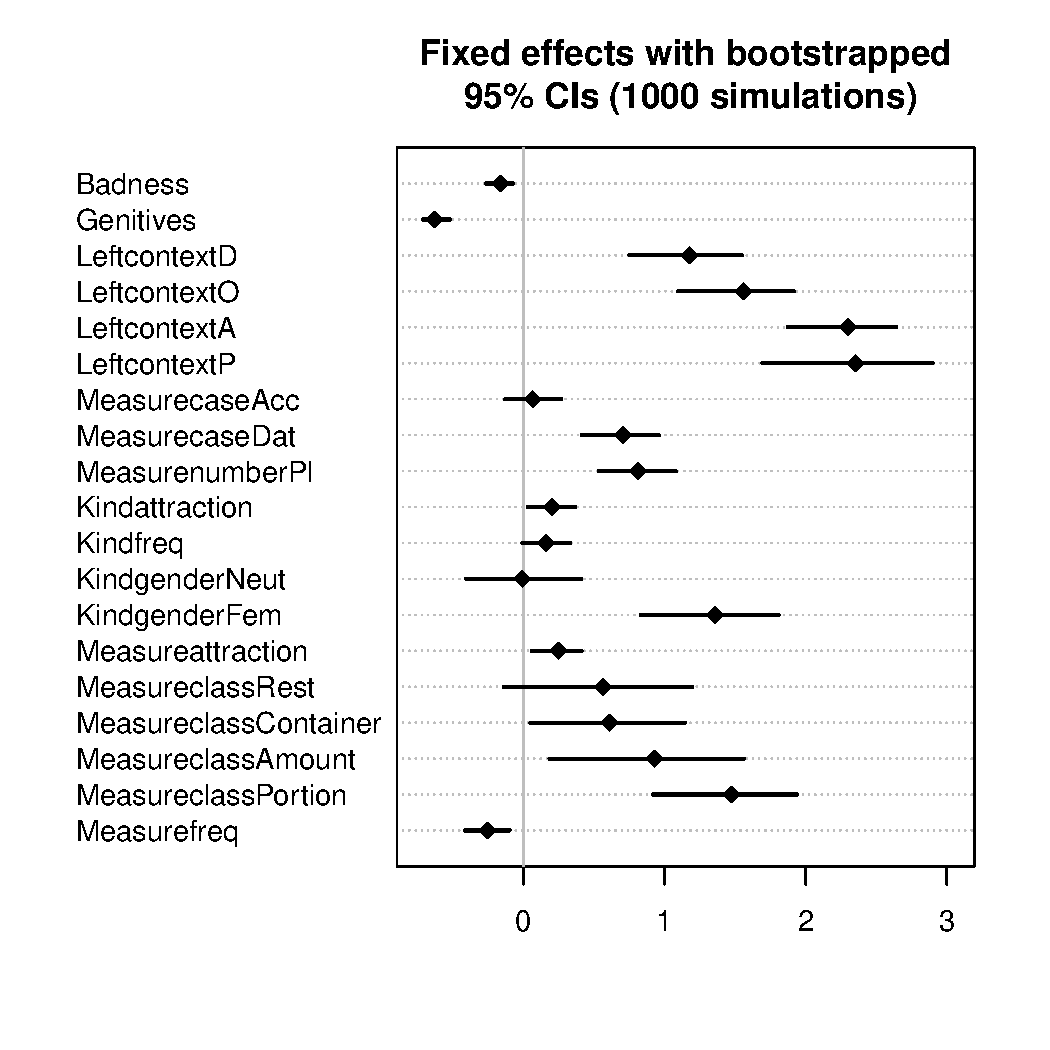
\includegraphics[width=0.85\textwidth]{../R/output/corpus_fixeffs}
  \caption{Coefficients (MLE) with 95\% parametric bootstrap confidence intervals; intercept (\textit{Leftcontext=C}, \textit{Measurecase=Nom}, \textit{Measurenumber=Sg}, \textit{Kindgender=Masc}, \textit{Measureclass=Physical}; 0 for all numeric z-transformed regressors) is -4.328}
  \label{fig:fixeffs}
\end{figure}

In this section, I report the results of fitting a multilevel model to the data using R \citep{R}, \textit{lme4} \citep{lme4} for Maximum Likelihood Estimation, and \textit{rstanarm} \citep{rstanarm} for Markov-Chain Monte Carlo estimation.
The purpose is to model the influence of the regressors specified in Table~\ref{tab:variables} on the probability that either the \NACa\ or the \PGCa\ is chosen.
All regressors from Table~\ref{tab:variables} were included to begin with, and the measure lemma and the kind noun lemma were specified as varying-intercept random effects.
The sample size was $n=5,063$ with $1,1344$ cases of \PGCa\ and $3,929$ cases of \NACa.
The results of the estimation are shown in Table~\ref{tab:bigtable} and in Figure~\ref{fig:fixeffs}.
The regressors with the measure lemma as their unit of reference have no within-measure lemma variance, and the \textit{glmer} function automatically estimates them as \textit{group level predictors} (or \textit{second-level effects}), cf.\ \cite[265--269,302--304]{GelmanHill2006}.
The same goes for those listed with the kind lemma as their unit of reference.
Given the coding of the response variable, coefficients leaning to the positive side can be interpreted as favouring the \PGCa.

\begin{sidewaystable}
  \centering
    \begin{tabular}{llrlrrrrrrcc}
      Level & Regressor & \multicolumn{1}{l}{\pPB} & Level  & \multicolumn{2}{l}{Coefficient} & \multicolumn{2}{l}{CI Low} & \multicolumn{2}{l}{CI High} & \multicolumn{2}{l}{CI contains 0} \\
              &                   &       &          & \multicolumn{1}{l}{MLE} & \multicolumn{1}{l}{MCMC} & \multicolumn{1}{l}{MLE} & \multicolumn{1}{l}{MCMC} & \multicolumn{1}{l}{MLE} & \multicolumn{1}{l}{MCMC} & \multicolumn{1}{l}{MLE} & \multicolumn{1}{l}{MCMC} \\\midrule

    First     & Badness           & 0.001 & (numeric) & -0.165 & -0.169 & -0.264 & -0.264 & -0.074 & -0.075 &      * &      * \\
              & Genitives         & 0.001 & (numeric) & -0.630 & -0.645 & -0.710 & -0.739 & -0.523 & -0.552 &      * &      * \\
              & Leftcontext       & 0.001 & D         &  1.178 &  1.173 &  0.751 &  0.784 &  1.548 &  1.546 &      * &      * \\
              &                   &       & O         &  1.561 &  1.588 &  1.093 &  1.179 &  1.919 &  2.007 &      * &      * \\
              &                   &       & A         &  2.300 &  2.340 &  1.872 &  1.959 &  2.644 &  2.726 &      * &      * \\
              &                   &       & P         &  2.353 &  2.371 &  1.693 &  1.766 &  2.900 &  2.978 &      * &      * \\
              & Measurecase       & 0.001 & Acc       &  0.065 &  0.070 & -0.130 & -0.119 &  0.268 &  0.269 &        &        \\
              &                   &       & Dat       &  0.707 &  0.735 &  0.413 &  0.480 &  0.959 &  1.002 &      * &      * \\
	      & Measurenumber     & 0.001 & Pl        &  0.814 &  0.825 &  0.534 &  0.574 &  1.080 &  1.079 &      * &      * \\[0.5\baselineskip]
                                          
    Second    & Kindattraction    & 0.033 & (numeric) &  0.204 &  0.216 &  0.030 &  0.014 &  0.366 &  0.412 &      * &      * \\
    (Kind)    & Kindfreq          & 0.066 & (numeric) &  0.161 &  0.173 & -0.008 &  0.009 &  0.333 &  0.350 &        &      * \\
              & Kindgender        & 0.001 & Neut      & -0.007 & -0.022 & -0.407 & -0.424 &  0.408 &  0.379 &        &        \\
	      &                   &       & Fem       &  1.357 &  1.379 &  0.831 &  0.872 &  1.808 &  1.897 &      * &      * \\[0.5\baselineskip]
                                          
    Second    & Measureattraction & 0.015 & (numeric) &  0.247 &  0.275 &  0.058 &  0.078 &  0.413 &  0.476 &      * &      * \\
    (Measure) & Measureclass      & 0.001 & Rest      &  0.564 &  0.488 & -0.140 & -0.309 &  1.197 &  1.236 &        &        \\
              &                   &       & Container &  0.609 &  0.618 &  0.050 &  0.018 &  1.145 &  1.215 &      * &      * \\
              &                   &       & Amount    &  0.927 &  0.959 &  0.184 &  0.189 &  1.566 &  1.718 &      * &      * \\
              &                   &       & Portion   &  1.472 &  1.503 &  0.916 &  0.956 &  1.938 &  2.064 &      * &      * \\
              & Measurefreq       & 0.003 & (numeric) & -0.257 & -0.264 & -0.413 & -0.435 & -0.098 & -0.099 &      * &      * \\
  \end{tabular}
  \smallskip
  \caption{Coefficient table comparing Maximum Likelihood Estimation (MLE, with 95\% bootstrap confidence interval) and `Bayesian' Markov-Chain Monte Carlo estimation (MCMC); for details see text}
  \label{tab:bigtable}
\end{sidewaystable}

Standard diagnostics for the Maximum Likelihood Estimation (MLE) show that the model quality is quite high.
Generalized variance inflation factors for the regressors were calculated to check for multicollinearity \citep{FoxMonette1992,ZuurEa2010}, and none of the corrected $\text{GVIF}^{1/2\text{df}}$ was higher than $2$.
Nakagawa \& Schielzeth's pseudo-coefficient of determination is $R_m^2=0.423$ and $R^2_c=0.515$ (see \citealp{Gries2015} for a linguist-friendly introduction to these $R^2$ measures, or else \citealp{NakagawaSchielzeth2013}).
The rate of correct predictions is $0.855$, which means a proportional reduction of error of $\lambda=0.354$.
The measure lemma intercepts have a standard deviation of $\sigma_{\text{Measurelemma}}=0.623$, the kind lemma intercept $\sigma_{\text{Kindlemma}}=0.488$.

The coefficient estimates are specified in Table~\ref{tab:bigtable} for each regressor (or regressor level) in the columns labelled \textit{Coefficient}.
For a robust quantification of the precision of the estimation, I ran a parametric bootstrap (using the \textit{confint.merMod} function from \textit{lme4}) with 1,000 replications, and using the percentile method for the calculation of the intervals.
The resulting 95\% bootstrap confidence intervals are reported in Table~\ref{tab:bigtable} in the columns labelled \textit{CI Low} and \textit{CI High} (= upper and lower 2.5th percentiles).
The column \textit{CI contains 0} shows an asterisk for those intervals that do \textit{not} include 0.
Furthermore, for each regressor, a $p$ value was obtained by dropping the regressor from the full model, re-estimating the nested model and comparing it to the full model.
Instead of inexact Wald approximations or Likelihood Ratio Tests, I used a drop-in bootstrap replacement for the Likelihood Ratio Test from the function \textit{PBmodcomp} from the \textit{pbkrtest} package \citep{HalekohHojsgaard2014}.
These bootstrapped $p$ values are given in the columns labelled p\Sub{PB} in Table~\ref{tab:bigtable}.
All regressors have low p\Sub{PB} values of magnitude $10^{-2}$ or $10^{-3}$.
Only \textit{Kindfreq} ($p_{\text{PB}}=0.066$) can be seen as slightly too high to be convincing (`non-significant').

Finally, I show that Bayesian methods in the form of Markov-Chain Monte Carlo estimation do not necessarily (and in this case predictably) lead to different results.
Both the MN model and the F model were re-estimated using the \textit{stan\_glmer} function from the \textit{rstanarm} package, which provides an \textit{lme4}-compatible syntax for estimating common model types with the \textit{stan} software \citep{CarpenterEa2017}.
The algorithm was run with $4$ chains and $1,000$ iterations, and instead of guessing prior distributions or using implausible uniform prior distributions \cite[251--252]{Levshina2016}, I used plausible default priors.
Most notably, priors for coefficients were specified as $\mathcal{N}(0,10)$ because coefficients higher than $10$ or lower than $-10$ are extremely rare in well-specified models on appropriate data.%
\footnote{Consider that with a coefficient of $10$, each increase by $1$ in the regressor variable means an increase in odds of $exp(10)=22,026.47$.
To reliably estimate such coefficients, extremely large samples would be required.}
The algorithm converged, and for all coefficients, the $\hat{R}$ diagnostic was exactly $1$.
The resulting coefficients and intervals as well as an * are also given in Table~\ref{tab:bigtable} in the columns labelled \textit{MCMC}.
Both methods lead to exactly the same results (minus negligible numerical differences) as expected (see Section~\ref{sec:rightstatistics}).
The signs and magnitudes of the coefficients are identical, and confidence intervals have the same width and symmetry properties.
If one were interested in significance at $\alpha=0.05$, then the decision based on the confidence intervals differs for \textit{Kindfreq} ($p_{\text{PB}}=0.066$, MLE lower bound is $-0.008$ and MCMC lower bound is $0.009$).
With MCMC, the regressor is `not significant' at the standard $\alpha$ level, but it is with MLE.
This might only go to show how absurd strict significance testing is in complex modelling situations:
both methods essentially estimate the same sign and magnitude for the coefficient (MLE $0.161$, MCMC $0.173$) and do not differ substantially with regard to the precision of the estimate in the form of the width of the confidence interval (both intervals have a width of exactly $0.341$).
Hence, I only interpret the MLE model in the next section.


%%%%%%%%%%%%%%%%%%%%%%%%%%%%%%%%%%%%%%%%%%%%%%%%%%%%%%%%%%%%%%%%%%%%%%%
%%%%%%%%%%%%%%%%%%%%%%%%%%%%%%%%%%%%%%%%%%%%%%%%%%%%%%%%%%%%%%%%%%%%%%%


\subsection{Interpretation}
\label{sec:interpretation}

% ATTRACTION

\begin{figure}[h!]
  \centering
  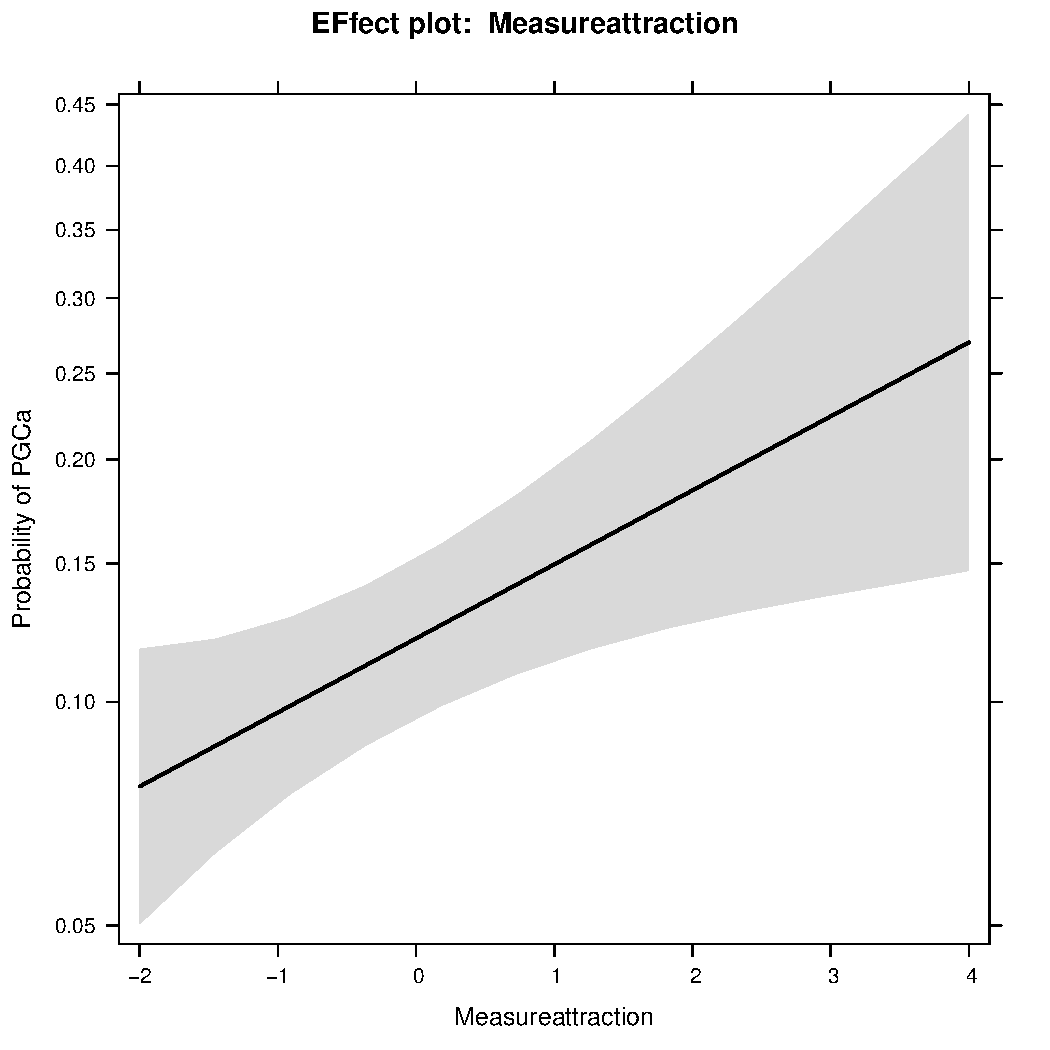
\includegraphics[width=0.5\textwidth]{../R/output/corpus_Measureattraction}~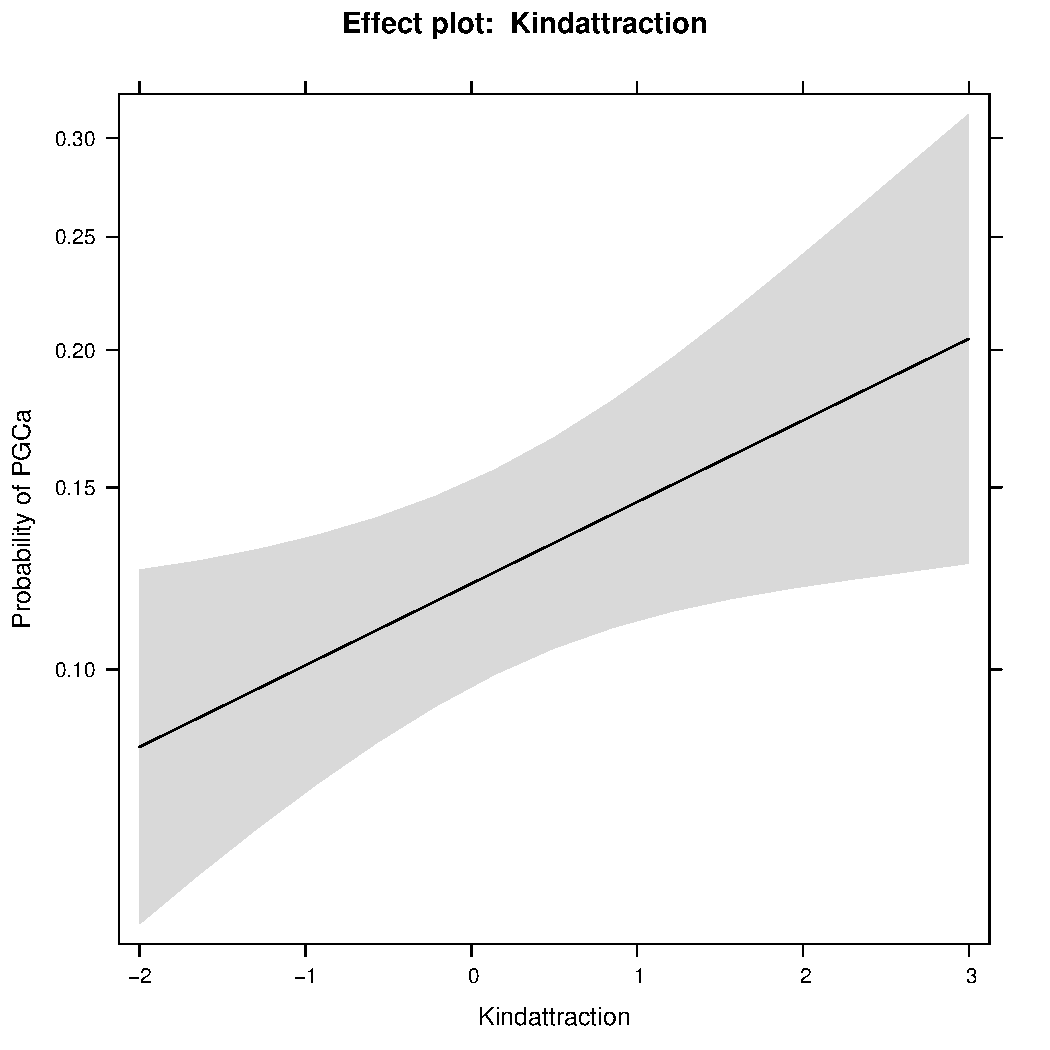
\includegraphics[width=0.5\textwidth]{../R/output/corpus_Kindattraction}
  \caption{Effect plots for the regressors \textit{Measureattraction} and \textit{Kindattraction}; y axes are not aligned}
  \label{fig:eff:attraction}
\end{figure}

The results reported in Section~\ref{sec:corpushierarchicalmodel} generally confirm the hypotheses from Section~\ref{sec:analyses}.
First, the prototypicality effect related to the non-alternating \PGCd\ and \NACb\ can be shown, see the effect plots in Figure~\ref{fig:eff:attraction}.%
\footnote{Effect plots were created using the \textit{effects} package \citep{Fox2003}.
They show the changes in probability for the outcome (y axis) dependent on values of a regressor (x axis), assuming typical values of all other regressors.}
The effect is mostly as expected:
if a lemma appears relatively more often in the \PGCd\ (compared to its frequency in the \NACb), the more often the \PGCa\ is chosen over the \NACa\ with this specific lemma.
The effect for measure nouns is stronger, and it was estimated with higher precision.


% GRAMMATICALISATION
% => lemmas and lemma classes

\begin{figure}[h!]
  \centering
  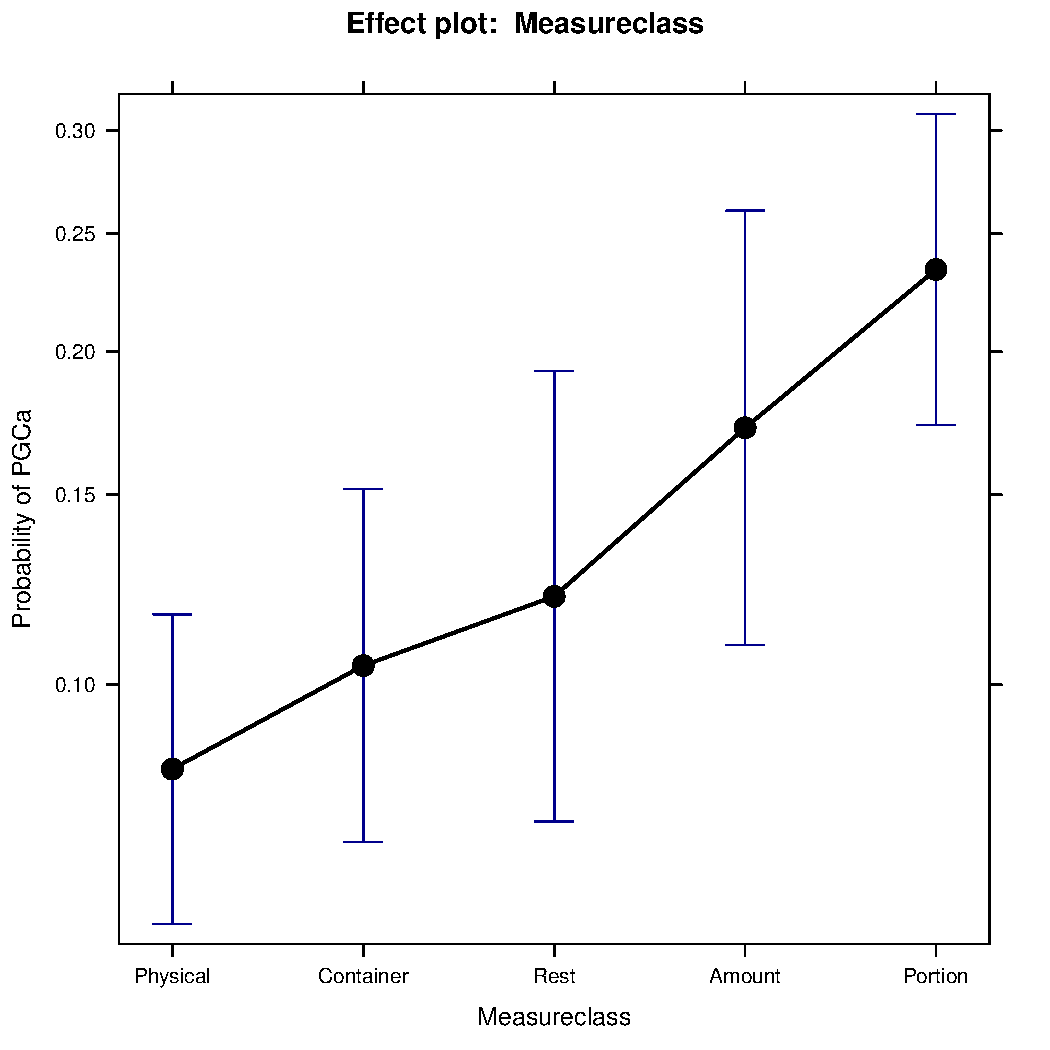
\includegraphics[width=0.75\textwidth]{../R/output/corpus_Measureclass}
  \caption{Effect plot for the regressor \textit{Measureclass}}
  \label{fig:eff:measureattraction}
\end{figure}

In Section~\ref{sec:analyses}, it was also hypothesised that there may be effects specific to classes of measure lemmas, and that they might be related to degrees of grammaticalisation of the measure noun.
Transcending the effects of individual lemmas (captured in the random intercepts), the \textit{Measureclass} second-level predictor was successfully estimated ($p_{\text{PB}}=0.001$).
Looking at the effect plot in Figure~\ref{fig:eff:measureattraction}, it is evident that abstract non-referential physical measure nouns (such as \textit{Gramm} `gram' or \textit{Liter} `litre') with a high degree of grammaticalisation favour the \NACa.
At the other end of the scale, nouns denoting natural portions like \textit{Haufen} `heap', \textit{Bündel} `bundle', \textit{Schluck} `gulp' favour the \PGCa.
These are referential nouns, confirming the hypothesis that it is prototypical of the PGC to host two referential nouns and the NAC only one.

% PLURAL & CARDINALS

\begin{figure}[h!]
  \centering
  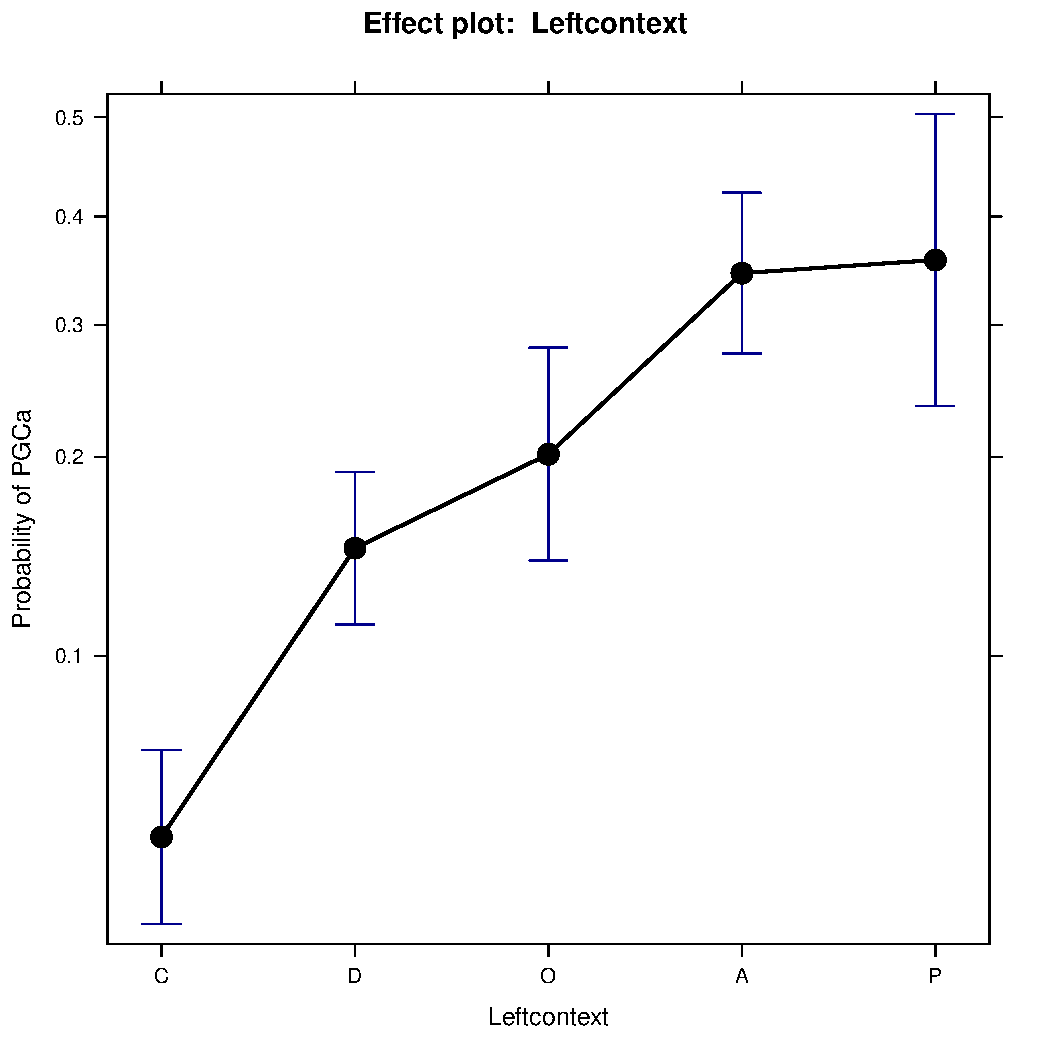
\includegraphics[width=0.75\textwidth]{../R/output/corpus_Leftcontext}
  \caption{Effect plot for the regressor \textit{Leftcontext}}
  \label{fig:eff:leftcontext}
\end{figure}

I now turn to the predicted effect of plural measure nouns and cardinals as quantifiers.
Plurality has a clear effect in the expected direction (plural favours the \PGCa) ($\beta_{\text{MeasurenumberPl}}=0.814$, $p=0.001$ for \textit{Measurenumber}).
Figure~\ref{fig:eff:leftcontext} shows that the left context of the measure noun influences the choice of the variant ($p=0.001$).
Cardinals have a strong tendency to co-occur with the \NACa\ in both models.

% REGISTER
% => Badness
% => Genitives

The register-related proxy variables point into the expected direction.
Increased \textit{Badness} of the document favours the \NACa\ ($\beta_{\text{Badness}}=-0.165$, $p=0.001$), and so does a lesser density of genitives ($\beta=-0.630$, $p=0.001$).
While these are poor proxies to register (and partially circular in the case of \textit{Genitives}), this result can at least encourage future work into register effects 

% NUISANCE
% => dative effect
% => frequency

The effect of \textit{Measurecase} ($p=0.001$) is as predicted by previous studies (see Section~\ref{sec:analyses}).
A measure noun in the dative favours the \PGCa\ with $\beta_{\text{MeasurecaseDat}}=0.707$ (compared to the nominative, which is on the intercept).
Although \textit{Measurecase} is a nuisance variable in the context of this study, convergence with previous work strengthens its validity.

%%%%%%%%%%%%%%%%%%%%%%%%%%%%%%%%%%%%%%%%%%%%%%%%%%%%%%%%%%%%%%%%%%%%%%%
%%%%%%%%%%%%%%%%%%%%%%%%%%%%%%%%%%%%%%%%%%%%%%%%%%%%%%%%%%%%%%%%%%%%%%%
%%%%%%%%%%%%%%%%%%%%%%%%%%%%%%%%%%%%%%%%%%%%%%%%%%%%%%%%%%%%%%%%%%%%%%%


\section{Experimental validation}
\label{sec:externalvalidation}

\subsection{Experiment 1: forced choice}

% TODO SURPRISAL
%
% Bybee, Joan und Thompson, Sandra. 1997. “Three Frequency Effects in Syntax”, Proceedings of the Twenty-Third Annual Meeting of the Berkeley Linguistics Society, 378-388.
% Bybee, Joan. 2006. “From Usage to Grammar: The Mind‘s Response to Repetition”. Language 82(4): 711-733.
% Levy, Roger .2008. “Expectation-based syntactic comprehension.” Cognition 106: 1126–1177.
% Smith, Nathaniel, and Levy, Roger. 2013. “The effect of word predictability on reading time is logarithmic.” Cognition 128: 302–319.

As was pointed out in Section \ref{sec:cogocl}, there is a strong interest in validating corpus-based findings through experiments in order to substantiate \textit{cognitively oriented usage-based corpus linguistics} as a research programme.
Therefore, this section and the next present the results of two experiments wherein I cross-checked the corpus-based findings.
Both experiments use attested sentences from the corpus sample (see Section~\ref{sec:gettingdata}) and the probabilities that the corpus-based statistical model (see Section~\ref{sec:corpushierarchicalmodel} assigns to the competing constructions in the sentences.
First, a forced-choice experiment was conducted.
Participants had to chose between two sentences differing only <++>

There were 24 participants (L1 speakers of German without reading or writing disability) aged 19 to 30 who were recruited from introductory linguistics courses at Freie Universität Berlin.
Although the experiment was conducted in the last four weeks of their first semester, participants had no deeper explicit knowledge of linguistics, grammar, or experimental methods.
None had never participated in a forced-choice experiment before.
Participation was voluntary, but participants received credit in partial fulfillment of course requirements.

As stimuli, attested (but simplified) sentences from the corpus study were used in an approach similar to the one taken in \cite{DivjakEa2016}.
I sampled 16 attested sentences from the corpus and simplified them (mostly removing embedded clauses, complex adverbials, etc.) and standardized their orthography.
It was made sure that the simplifications and normalisations did not affect any of the regressors used in the corpus study.
Eight sentences contained masculine or neuter kind nouns, the other eight contained feminine kind nouns.
Furthermore, in each of the M\slash N and F groups, four sentences with a case drop (\ie\ genitive or oblique case on the kind noun) and four withe case identity were chosen.
More precisely, the four sentences were sampled as highly prototypical examples of case drop (high logits) and case identity (low logits), respectively, according to the corpus based models.%
\footnote{Sentences were sorted by their corresponding $\hat{y}$ calculated from the model.
For the M\slash N sentences, sentences were sampled from the top and bottom 15\% of the resulting vector.
For the F sentences, the top and bottom 25\% were used because the overall sample size was smaller.}
It was made sure that the highly predictive features according to Section \ref{sec:interpretation} occurred in unique combinations among the four sentences in each cell.
The design is summarised in Table \ref{tab:experiment1:design}.

\begin{table}
  \centering
  \begin{tabular}[h]{rcc}
     & M\slash N & F \\
     \midrule
     \textbf{high prob.\ for case drop} & 4 sentences\Supsf{a} & 4 sentences\Supsf{a} \\
     \textbf{low prob.\ for case drop} & 4 sentences\Supsf{a} & 4 sentences\Supsf{a} \\
  \end{tabular}
  \caption{The four groups of attested sentences chosen as stimuli (\Supsf{a}Among the 4 sentences, combinations of important factor values were made unique.)}
  \label{tab:experiment1:design}
\end{table}

The pairs of stimuli were the original attested sentence containing the preferred construction and a modified version containing the dispreferred construction.
They were presented next to each other, and a 20 second time limit for each choice was set.%
\footnote{No participant ever exceeded the time limit.}
The position on the screen (left\slash right) and the order of sentences were randomized for each participant.
As fillers, 23 pairs of sentences exemplifying similar alternation phenomena from German morpho-syntax were used.
Thus, participants saw 39 pairs of sentences and 78 sentences in total.
They were instructed to select from each pair of sentences the one that seemed more natural to them in the sense that they would use it rather than the other one.
The experiment was conducted using \textit{PsychoPy} \citep{Peirce2007}.

\begin{figure}[h]
\centering
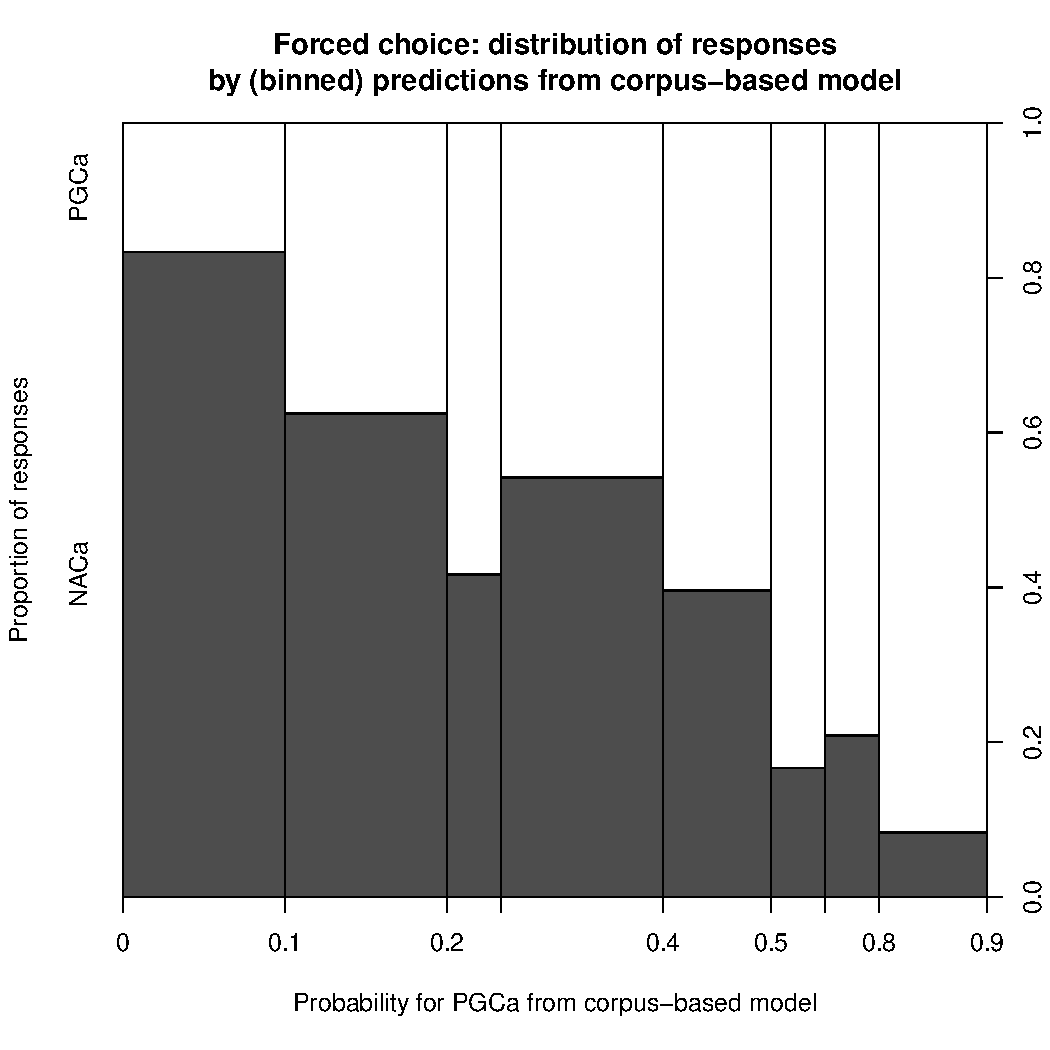
\includegraphics[width=0.75\textwidth]{../R/output/fc_proportions}
\caption{Participants' responses in the forced-choice task plotted against the predictions from the corpus-based model}
\label{fig:afc:proportions}
\end{figure}

Figure \ref{fig:afc:proportions} shows the relationship between the logits calculated from the corpus-based model and the proportional choices made by participants.
Visually, it looks like there is a close correlation between the corpus-derived preferences and preferences in the forced choice experiment.

Then, a multilevel logistic regression was specified.
Coefficients were estimated using Maximum Likelihood, and the coefficient table is given in Table \ref{tab:afc:model}, where instead of approximate standard errors and $z$ and $p$ values the lower and the upper bound of a bootstrapped 95\% confidence interval are specified.

\begin{table}
  \centering
  \begin{tabular}{lrrr}
    Effect & Estimate & 95\% CI lower & 95\% CI upper \\
    \midrule
    (Intercept)            &  0.748  &  0.242  &  1.265 \\
    Modelpred              &  1.154  &  0.905  &  1.497 \\
    KindgenderMN           &  0.135  & -0.416  &  0.632 \\
    Modelpred:KindgenderMN & -0.567  & -0.843  & -0.298 \\
  \end{tabular}
  \caption{Coefficient table for the GLMM specified in equation \ref{eq:model:afc}, analysing the results of the forced choice experiment}
  \label{tab:afc:model}
\end{table}

The number of observations was $n=768$.
The random effects for participant ($\sigma=0.7841$, 24 groups) and item ($\sigma=0.4869$, 16 groups) show considerable variance.
Accordingly, there is a notable difference between the marginal and conditional Nakagawa \& Schielzeth's $R^2_{m}=0.383$ and $R^2_{c}=0.510$, while both values are quite high.
Dropping the term of interest ($\beta^1\cdot x_i^1+\beta^2\cdot x_i^2+\beta^{1.2}\cdot x_i^1\cdot x_i^2$) leads to a significantly worse fit of the nested model both in a traditional Likelihood Ratio Test ($LR=55.172$, $p<0.0001$) and its bootstrapped PB alternative ($p = 0.002$, 493 of 500 requested samples used).
The effect display for the term is given in Figure \ref{fig:afc:effects}.

\begin{figure}[h]
\centering
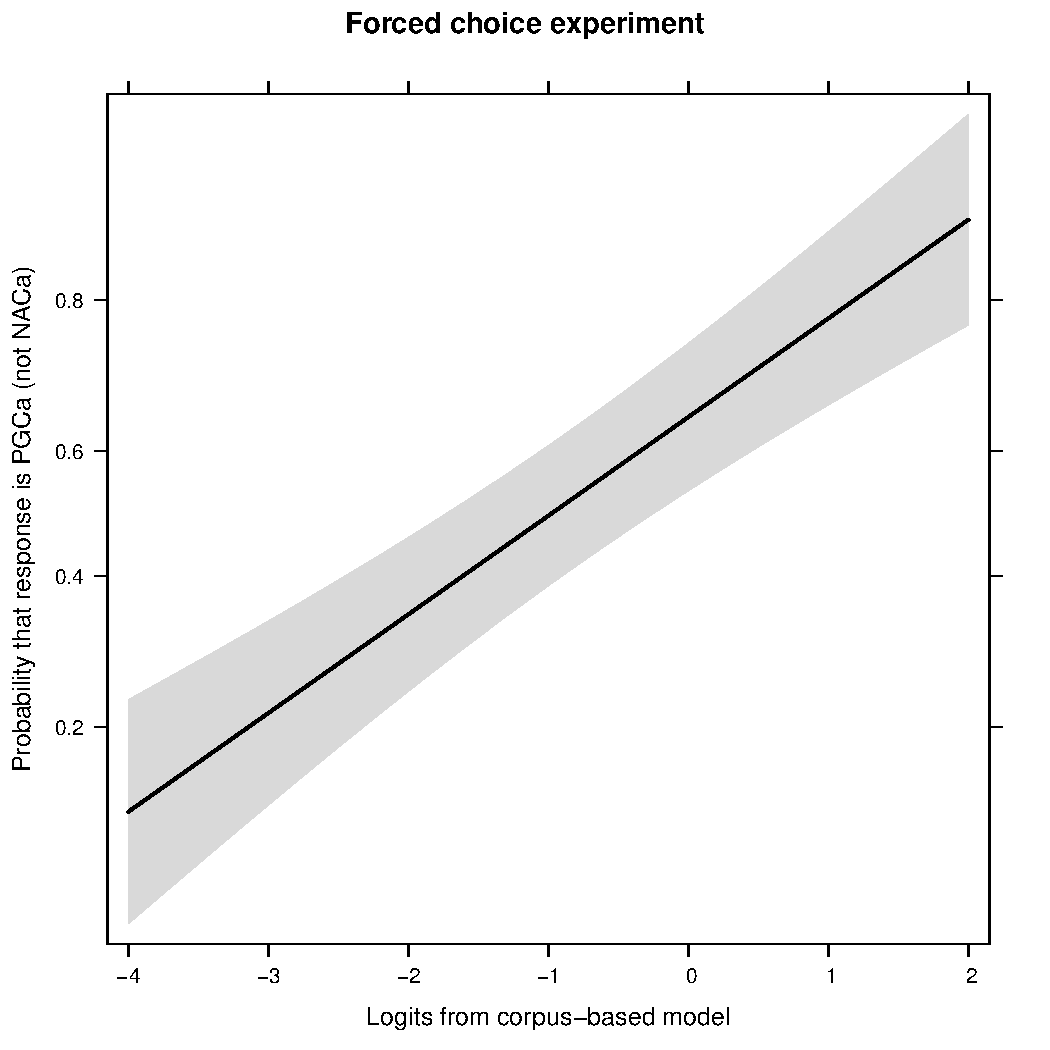
\includegraphics[width=0.75\textwidth]{../R/output/fc_effects}
\caption{Effect plot for the multilevel logistic regression in the forced-choice experiment: predictability of participants' choices from the logits of the corpus-based GLMM (cf.\ Section~\ref{sec:corpushierarchicalmodel})}
\label{fig:afc:effects}
\end{figure}

In summary, the forced choice experiment clearly succeeded in validating the results from the corpus study in as much as the preferences extracted from the corpus correspond to native speakers' choices.
We can take this as an indication that there is some relation between the process generating the corpus data and the behaviour of individual speakers.
In the next section, I report the results of a self-paced reading experiment which yielded (maybe expectedly) less clear results.



%%%%%%%%%%%%%%%%%%%%%%%%%%%%%%%%%%%%%%%%%%%%%%%%%%%%%%%%%%%%%%%%%%%%%%%
%%%%%%%%%%%%%%%%%%%%%%%%%%%%%%%%%%%%%%%%%%%%%%%%%%%%%%%%%%%%%%%%%%%%%%%

\subsection{Experiment 2: self-paced reading}

%\begin{figure}[h]
%\centering
%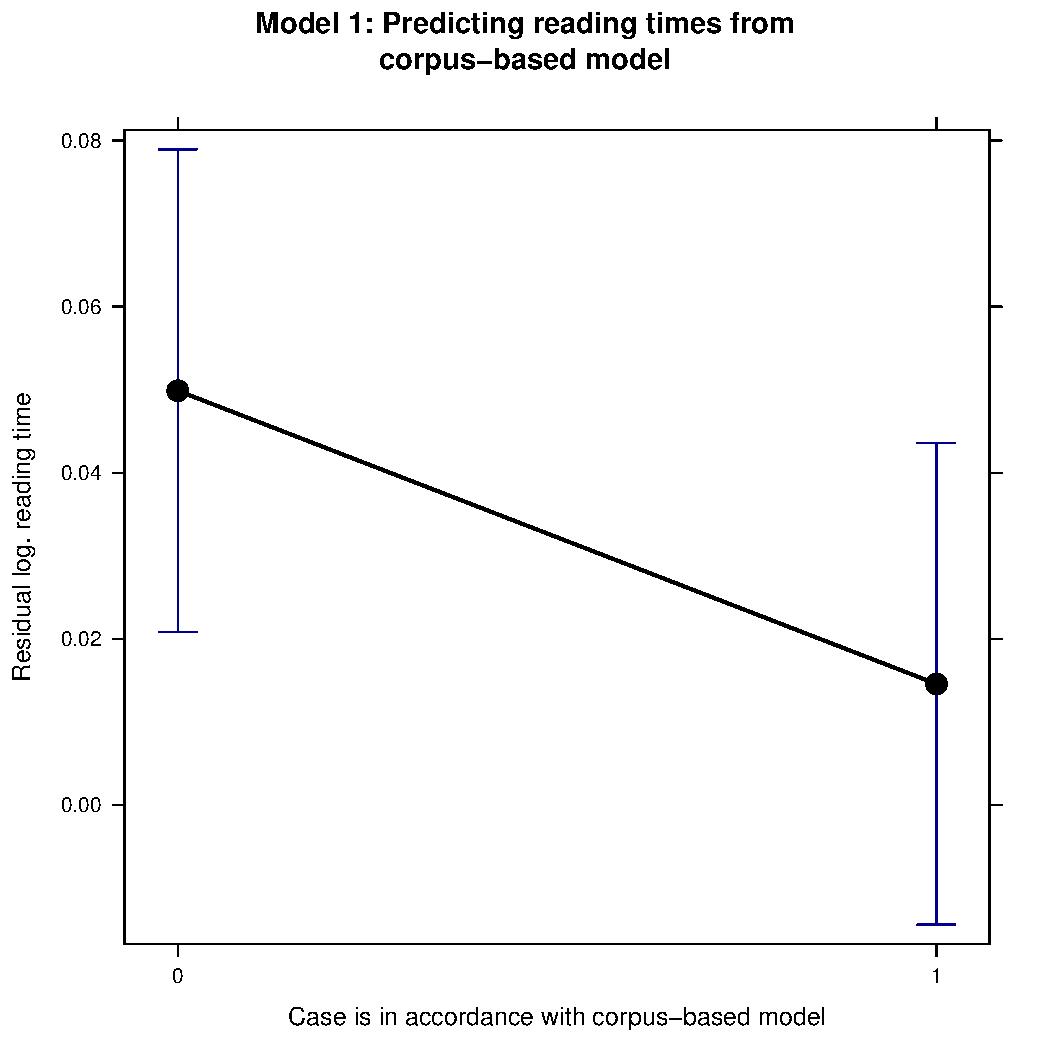
\includegraphics[width=0.6\textwidth]{figures/experiment/spr_effects_modelPredDichotomousReg}
%\caption{Effect plot for the LMM in the self-paced reading experiment: modeling participants' residualised log reading times on the dichotomised predictions of the corpus-based GLMM (cf.\ Section~\ref{sec:corpushierarchicalmodel})}
%\label{fig:spr:dichotomous:effects}
%\end{figure}

\begin{figure}[h]
\centering
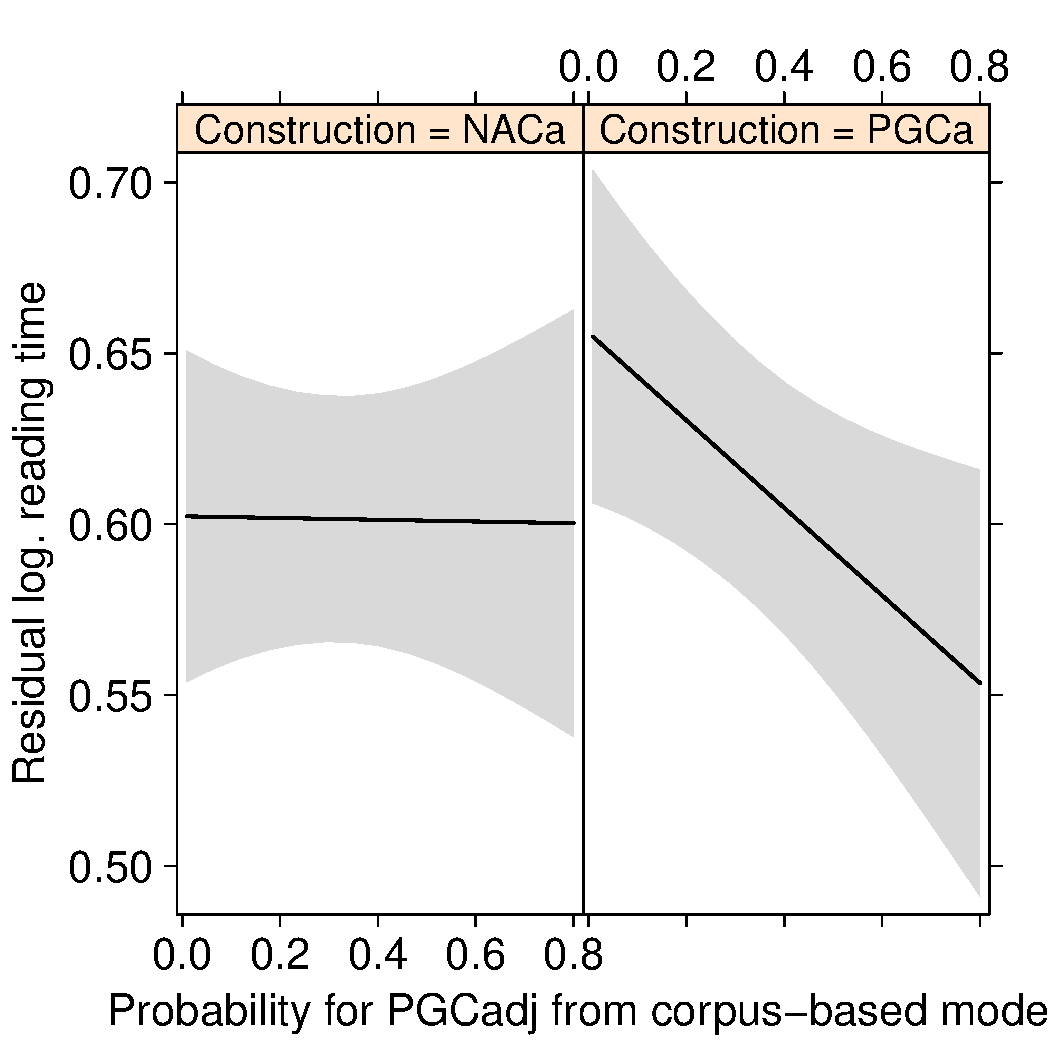
\includegraphics[width=0.75\textwidth]{../R/output/spr_effects}
\caption{Effect plot for the LMM in the self-paced reading experiment: modeling participants' residualised log reading times on the predictions (logits) of the corpus-based GLMM (cf.\ Section~\ref{sec:corpushierarchicalmodel})}
\label{fig:spr:continuous:effects}
\end{figure}



%%%%%%%%%%%%%%%%%%%%%%%%%%%%%%%%%%%%%%%%%%%%%%%%%%%%%%%%%%%%%%%%%%%%%%%
%%%%%%%%%%%%%%%%%%%%%%%%%%%%%%%%%%%%%%%%%%%%%%%%%%%%%%%%%%%%%%%%%%%%%%%
%%%%%%%%%%%%%%%%%%%%%%%%%%%%%%%%%%%%%%%%%%%%%%%%%%%%%%%%%%%%%%%%%%%%%%%


\section{Conclusions}





%%%%%%%%%%%%%%%%%%%%%%%%%%%%%%%%%%%%%%%%%%%%%%%%%%%%%%%%%%%%%%%%%%%%%%%
%%%%%%%%%%%%%%%%%%%%%%%%%%%%%%%%%%%%%%%%%%%%%%%%%%%%%%%%%%%%%%%%%%%%%%%
%%%%%%%%%%%%%%%%%%%%%%%%%%%%%%%%%%%%%%%%%%%%%%%%%%%%%%%%%%%%%%%%%%%%%%%
%%%%%%%%%%%%%%%%%%%%%%%%%%%%%%%%%%%%%%%%%%%%%%%%%%%%%%%%%%%%%%%%%%%%%%%



\begin{acknowledgement}
  I want to thank (in alphabetical order) Felix Bildhauer, Götz Keydana, and Ulrike Sayatz for stimulating discussions on relevant aspects of this paper.
  I also thank Ulrike Sayatz for recruiting the participants for the experiments.
  I am grateful to Kim Maser for her work on the annotation of the concordances.
  Furthermore, Samuel Reichert substantially helped to develop the guiding ideas behind this study by writing an excellent BA theses on the subject under my supervision.
  The research presented here was made possible in part through funding from the \textit{Deutsche Forschungsgemeinschaft} (DFG, personal grant SCHA1916/1-1).
\end{acknowledgement}



%%%%%%%%%%%%%%%%%%%%%%%%%%%%%%%%%%%%%%%%%%%%%%%%%%%%%%%%%%%%%%%%%%%%%%%
%%%%%%%%%%%%%%%%%%%%%%%%%%%%%%%%%%%%%%%%%%%%%%%%%%%%%%%%%%%%%%%%%%%%%%%
%%%%%%%%%%%%%%%%%%%%%%%%%%%%%%%%%%%%%%%%%%%%%%%%%%%%%%%%%%%%%%%%%%%%%%%
%%%%%%%%%%%%%%%%%%%%%%%%%%%%%%%%%%%%%%%%%%%%%%%%%%%%%%%%%%%%%%%%%%%%%%%


\bibliography{rs,cow}
\end{document}



%\footnote{\cite{AnttilaFong2000} propose an \textit{Obligatory Contour Principle for case} (Case-OCP) in a superficially similar but fundamentally unrelated case alternation in Finnish partitives.
%}
%
% On Case-OCP (from Götz Keydana):
% Und da habe ich dann auch einen Verweis auf den locus classicus gefunden:
% STEFAN A. FRISCH, JANET B. PIERREHUMBERT and MICHAEL B. BROE: SIMILARITY AVOIDANCE AND THE OCP. Natural Language & Linguistic Theory 22: 179–228, 2004.
% Dazu gäbe es dann noch, ebenfalls von Pierrehumbert,
% Dissimilarity in the Arabic Verbal Roots. In Amy Schafer, ed.,Proceedings of NELS 23 Amherst, MA: Graduate Linguistics Student Association. 1993. pp 367-381 
% Darin stellt sie wohl erstmals explizit einen Zusammenahng zwischen OCP und Kognition her.
